



\documentclass[12pt]{article}

% ============================================================================
% AER-Style Preamble
% ============================================================================
\usepackage{fontspec}
\usepackage{unicode-math}
\setmainfont{Times New Roman}
\setmathfont{Cambria Math}
\usepackage{amsmath,amsthm}  % amssymb removed: unicode-math already provides all its symbols
\usepackage{graphicx}
\usepackage{booktabs}
\usepackage{natbib}
% setspace not available; use linespread instead
\usepackage[margin=1in]{geometry}
\usepackage{caption}
\usepackage{subcaption}
\usepackage{float}
\usepackage{hyperref}
\usepackage{xcolor}
\usepackage{multirow}
\usepackage{array}
\usepackage{threeparttable}
\usepackage{rotating}
\usepackage{pdflscape}
\usepackage{enumitem}
\usepackage{placeins}
\usepackage{indentfirst}

\hypersetup{colorlinks=true, linkcolor=blue!60!black, citecolor=blue!60!black, urlcolor=blue!60!black}
\captionsetup{font=small, labelfont=bf, labelsep=period}

\linespread{1.5}  % 1.5 line spacing for Energy Economics submission
\setlength{\parindent}{1.5em}
\setlength{\parskip}{0pt}

\newtheorem{proposition}{Proposition}
\newtheorem{corollary}{Corollary}

% ============================================================================
% Title Page
% ============================================================================

\title{The Cost of Closing the Strait of Hormuz: A DSGE Analysis\thanks{This paper builds on the empirical framework of \citet{federle2026price}. We thank seminar participants for helpful comments. All errors are our own.}}

\author{
  \textsc{Weijia Wang}\thanks{Corresponding author. School of Economics and Finance, Xi'an Jiaotong University, Xi'an, Shaanxi 710000, China. Email: \href{mailto:wangweijia@stu.xjtu.edu.cn}{wangweijia@stu.xjtu.edu.cn}. Ph.D.\ candidate, School of Economics and Finance, Xi'an Jiaotong University. Research interests: international economics and energy policy.}
  \and
  \textsc{Wenli Xu}\thanks{School of Finance, City University of Macau, Macau, China. Email: \href{mailto:wlxu@cityu.edu.mo}{wlxu@cityu.edu.mo}. ORCID: \href{https://orcid.org/0009-0007-0676-7359}{0009-0007-0676-7359}.}
}

\date{April 2026}

\begin{document}

\maketitle

\begin{abstract}
We construct a four-region New Keynesian DSGE model to quantify the global macroeconomic costs of a Strait of Hormuz blockade, integrating oil-supply, trade, financial contagion, stabilization-policy, expectation, and fiscal channels within a unified framework. In the baseline calibration, a blockade raises global oil prices by 64.2 percent, pushes Iran's output gap to $-34.1$ percentage points, and generates a global consumption-equivalent welfare loss index of 0.485 percentage points. China's triple stabilization combines strategic petroleum reserve releases, renewable-energy substitution, and manufacturing export expansion. It reduces the oil-price peak by 5.0 percentage points and lowers global welfare losses by 0.045 percentage points, but an endogenous OPEC+ supply response is the larger marginal stabilizer: high OPEC+ activation combined with China's instruments cuts the global loss to 0.347 percentage points. Disaggregating the rest of the world reveals that oil exporters are nearly insulated (0.039 percentage-point loss) while oil importers bear a 0.786 percentage-point loss obscured by the aggregate ROW block. Severe Gulf-infrastructure escalation more than doubles the oil-price spike to 126.6 percent and raises global welfare loss to 0.731 percentage points. Pre-war anticipation redistributes losses intertemporally without materially changing their total, but successful diplomacy is worth 0.204 percentage points of global permanent consumption. Inflation-expectation de-anchoring and fiscal debt sustainability, rather than conventional Taylor-rule activism, emerge as the binding second-round policy risks.

\bigskip
\noindent \textbf{JEL Codes:} E32, F41, F51, H56, Q43 \\
\noindent \textbf{Keywords:} Strait of Hormuz, DSGE, oil supply shocks, financial contagion, China stabilization, geopolitical risk, energy security
\end{abstract}

\thispagestyle{empty}
\newpage
\setcounter{page}{1}

% ============================================================================
% I. INTRODUCTION
% ============================================================================

\section{Introduction}

The Strait of Hormuz carries roughly 20 percent of global petroleum trade through a navigable channel less than three kilometers wide at its narrowest point. A sustained blockade would represent the largest single-point disruption to global oil supply ever recorded, yet the structural macroeconomics literature has no quantitative model of what such a closure would cost, or through which channels those costs would propagate. \citet{federle2026price} document that wars reduce war-site GDP by roughly 10 percent and generate third-country spillovers through bilateral trade, but their reduced-form local projections cannot trace the energy-price, financial-contagion, and stabilization channels that activate when a single geographic chokepoint seizes global commodity flows. The central question this paper addresses is therefore not merely quantitative but structural: \textit{to what extent does sovereign credit risk network contagion amplify traditional trade-channel losses when a single geographic chokepoint disrupts global oil flows?} The question is not answered by reduced-form estimates because the amplification mechanism---a geopolitical shock propagating through sovereign-spread dynamics to compress investment and output in economies that have negligible bilateral trade with the war site---requires a framework in which financial linkages across borders are explicitly modeled, their magnitudes are disciplined by historical evidence, and their interaction with the oil-supply shock can be isolated from the trade channel. Nor can existing two-country DSGE models answer the policy counterfactuals that motivate current energy-security planning: Does aggressive monetary easing help or hurt when the inflation source is a supply shock amplified by financial contagion? Would a Chinese strategic stabilization effort matter, and if so, through which specific margin?

We answer these questions with a four-region New Keynesian DSGE model calibrated to a Hormuz-blockade scenario triggered by regional military escalation. The four regions, Iran (the war site), the US--Israel bloc (the external-belligerent aggregate), China (the major oil-importing stabilizer), and the rest of the world (ROW), are each governed by a standard New Keynesian three-equation system and linked through a global oil market, bilateral trade flows, and a financial contagion matrix whose off-diagonal entries are disciplined by the historical sovereign-spread dynamics documented in Section~\ref{sec:facts}. The US--Israel label denotes an aggregate military-demand and safe-haven block quantitatively dominated by the US economy, not a separate structural model of two distinct countries. Around this baseline, we employ six mechanism-verification exercises that each isolate one amplification or attenuation channel: spare supply capacity (OPEC+), distributional heterogeneity within the third-country block, escalation nonlinearity, financial pre-adjustment under anticipation, inflation-expectation persistence, and fiscal-financial feedback. These exercises are not independent stress tests but a coherent identification strategy: by varying the financial and institutional environment while holding the core chokepoint structure fixed, they demonstrate that sovereign credit risk network contagion is the dominant amplifier of trade-channel losses across all configurations studied, and that the welfare ranking of stabilization instruments is preserved regardless of which secondary channel is activated.

The structural analysis delivers three sets of quantitative findings that cannot be recovered from reduced-form estimates. The baseline blockade raises global oil prices by 64.2 percent and generates a global welfare loss of 0.485 percentage points of permanent consumption. China's triple stabilization combines strategic petroleum reserve releases, renewable-energy substitution, and manufacturing export expansion, reducing the oil-price peak by approximately five percentage points and saving 0.045 percentage points of global welfare. A full OPEC+ spare-capacity response combined with China's instruments saves 0.183 percentage points and reduces the oil-price peak to 56.9 percent. The operative stabilizing margin is therefore spare physical production capacity acting directly on the missing-barrel supply gap, not demand-side reserve drawdowns. Disaggregating the rest-of-world block into net oil exporters and importers reveals that the aggregate ROW welfare figure conceals opposite-signed effects: exporters lose only 0.039 percentage points while importers bear a 0.786 percentage-point loss, a distributional gap of 0.578 percentage points hidden by the aggregate 0.617 figure, and policy prescriptions calibrated to the aggregate would systematically misattribute commodity windfall gains to exporters as evidence of general third-country resilience. Escalation intensity, inflation-expectation anchoring, and pre-existing fiscal space determine the tail: moderate Gulf-infrastructure damage raises the oil-price peak to 95.4 percent while severe damage raises it to 126.6 percent and global welfare losses to 0.731 percentage points. Pre-war anticipation redistributes losses intertemporally without materially changing their total, while successful diplomacy avoids 0.204 percentage points of global loss. Under severe expectation de-anchoring, aggressive Taylor-rule tightening worsens welfare by amplifying the output contraction without reducing the cost-push source of inflation, and the US--Israel bloc breaches the 130 percent debt-to-GDP sustainability threshold under every fiscal rule examined, indicating that pre-existing fiscal space rather than crisis-era activism is the operative constraint.

Four strands of prior work inform the analysis. The economics of war and conflict provides the foundational empirical anchor. Using a comprehensive dataset of armed conflicts since 1870, \citet{federle2026price} document that wars reduce war-site GDP by roughly 10 percent on average and that third-country spillovers flow primarily through bilateral trade exposure, with each percentage point of bilateral trade share generating approximately 0.5 percentage points of spillover output loss. Their reduced-form local projections identify these average effects cleanly but cannot decompose them into the energy-price, financial, and supply-chain components that activate in a chokepoint scenario, and the Hormuz case is precisely the outlier their cross-war average is not designed to capture: bilateral Iran--importer trade is far too small, at most 1.5 percent of China's imports, to account for the large third-country losses the model generates, which instead flow through the global oil-price channel activated by the chokepoint geometry. \citet{abadie2003economic} establish the synthetic-control methodology for conflict-cost estimation that informs the construction of our no-war counterfactual path; \citet{barro2006rare} provides the rare-disaster framework that motivates pricing tail-risk welfare losses through a discounted consumption-equivalent index rather than relying on local linear approximations around a steady state.

The structural modeling of geopolitical and energy shocks constitutes the second strand. \citet{caldara2022measuring} construct a monthly index of geopolitical risk from automated newspaper text searches and use it to identify geopolitical risk shocks in vector autoregressions on U.S. and international data. Their central finding that geopolitical risk shocks depress industrial production, employment, and stock returns while generating capital outflows from emerging economies toward safe havens motivates the central position of the financial contagion matrix in the present framework and directly disciplines the calibration of $\gamma_s$ and $\gamma_k$ in the financial conditions index~(\ref{eq:fci}). The same evidence shows that financial-market transmission quantitatively dominates bilateral goods-trade linkages. \citet{caldara2022measuring} further demonstrate that both geopolitical threats and geopolitical acts contribute independently to economic outcomes, a finding directly tested in the news-shock extension of Section~\ref{sec:news}, which separates the financial costs of anticipation from the physical costs of blockade. \citet{bodenstein2011oil} develop the two-country open-economy New Keynesian DSGE with oil that we extend from two to four regions; their calibration of short-run demand and supply price elasticities, $|\varepsilon_d| = 0.05$ and $\varepsilon_s = 0.10$, carries directly into our oil-price equation~(\ref{eq:oil_price}), and their analysis of asymmetric exporter--importer responses provides the structural rationale for the ROW disaggregation in Section~\ref{sec:row_split}. The extension from two to four regions matters substantively: the two-country structure forces Iran and the global oil market into the same region, obscuring the chokepoint mechanism, whereas a separate war-site region allows the simultaneous supply-destruction and revenue-loss dynamics to generate stagflation at their full empirical intensity while transmitting the oil-price shock to the remaining three regions.

The energy economics of supply disruptions provides the quantitative discipline for the oil-market specification. \citet{hamilton1983oil} establishes the foundational regularity that oil supply disruptions cause recessions, and the time-series evidence in \citet{hamilton2009understanding} documents that crude oil demand is highly price-inelastic at acute-disruption horizons, approximately $-0.06$ over one year, while supply is equally unresponsive. These estimates rationalize the $|\varepsilon_d| = 0.05$ and $\varepsilon_s = 0.10$ values in equation~(\ref{eq:oil_price}) and explain why even a partial chokepoint blockade translates into a disproportionately large price spike: with an elasticity denominator of only 0.15, a 10 percent supply shortfall generates a price increase of roughly 67 percent before reserve releases and demand feedback. \citet{kilian2009not} introduces the identification refinement that the macroeconomic consequences of oil price increases depend on whether they originate from supply disruptions, global demand expansions, or precautionary demand; correctly distinguishing the source matters for monetary policy because a supply-driven increase generates simultaneous output contraction and cost-push inflation, making Taylor-rule tightening potentially counterproductive. This is precisely the configuration explored in Section~\ref{sec:deanchoring}. \citet{blanchard2007macroeconomic} document that oil shock effects have diminished since the 1980s due to reduced energy intensity, improved monetary credibility, and more flexible factor markets; their framework motivates the region-specific $\alpha_{e,i}$ parameters that generate heterogeneous pass-through in equations~(\ref{eq:nkpc}) and~(\ref{eq:is}), and the monetary-credibility dimension of the de-anchoring extension.

China's global stabilization role and the mechanics of financial contagion constitute the fourth strand. \citet{zhang2020china} develop a closed-economy DSGE model of China's strategic petroleum reserve and document that coordinated SPR releases reduce oil-price volatility: a release equivalent to 0.5 percent of global supply reduces the oil price by roughly three to five percentage points, consistent with the approximately five-percentage-point reduction estimated in the baseline. We extend their analysis by embedding the SPR in a four-region global framework that recovers the public-good externality of reserve policy accruing to all net-importing regions, and by adding the renewable substitution and manufacturing channels that reveal the SPR to be the capacity-constrained instrument while manufacturing remains unconstrained throughout the blockade window. \citet{helveston2019china} document that China's solar photovoltaic supply chain has reduced global module costs by 24 percent over the past decade through economies of scale and competitive specialization; the same mechanism applies to the manufacturing export channel in equation~(\ref{eq:mfg}), where industrial reorientation toward disrupted supply gaps generates disinflationary spillovers to trading partners proportional to their trade openness $\omega_i$. \citet{longstaff2011financial} demonstrate that sovereign credit risk transmits across borders through portfolio rebalancing and risk-appetite channels independently of bilateral trade or financial exposure, providing the empirical foundation for the off-diagonal entries of the financial linkage matrix~(\ref{eq:linkage_matrix}) and for the risk-aversion amplifier $\Gamma_t$ that intensifies contagion during capital flight from the war site. \citet{rey2015dilemma} documents that the global financial cycle drives co-movement in capital flows and credit conditions across economies with negligible direct bilateral links, undermining floating exchange rates as shock absorbers, a finding that motivates both China's FX intervention term in equation~(\ref{eq:rer}) and the partial capital-account insulation that differentiates China's financial transmission from the broader ROW block.

Section~\ref{sec:facts} documents the stylized facts motivating the scenario. Sections~\ref{sec:model}--\ref{sec:calibration} present the model and calibration. Section~\ref{sec:results} reports baseline results. Section~\ref{sec:robustness} presents the six extensions. Section~\ref{sec:conclusion} draws policy implications.

% ============================================================================
% II. STYLIZED FACTS: THE STRAIT OF HORMUZ AS GLOBAL CHOKEPOINT
% ============================================================================

\section{Stylized Facts: The Strait of Hormuz as a Global Chokepoint}
\label{sec:facts}

Before presenting the model, we document five stylized facts that motivate both the scenario and its transmission channels. These facts collectively establish three premises: the Strait of Hormuz is uniquely irreplaceable among global oil-transit nodes; the economies that depend on it are large, concentrated, and highly exposed; and historical episodes confirm that Middle East conflicts transmit to global financial markets well beyond their bilateral trade footprints.

The first fact is the physical concentration of oil transit. Figure~\ref{fig:chokepoints} ranks the world's major oil-transit chokepoints by daily volume. The Strait of Hormuz carries 21 million barrels per day, approximately 20 percent of global petroleum trade, roughly 30 percent more than the next-largest chokepoint (the Strait of Malacca at 16 mbd) and more than double the Suez Canal. Critically, it has no practical bypass: the Abqaiq--Yanbu pipeline can redirect at most 5 mbd of Saudi crude, leaving 16 mbd with no alternative route. This asymmetry means a blockade cannot be circumvented at scale within the time horizon of the shock, a modeling assumption our scenario embeds directly.

\begin{figure}[H]
\centering
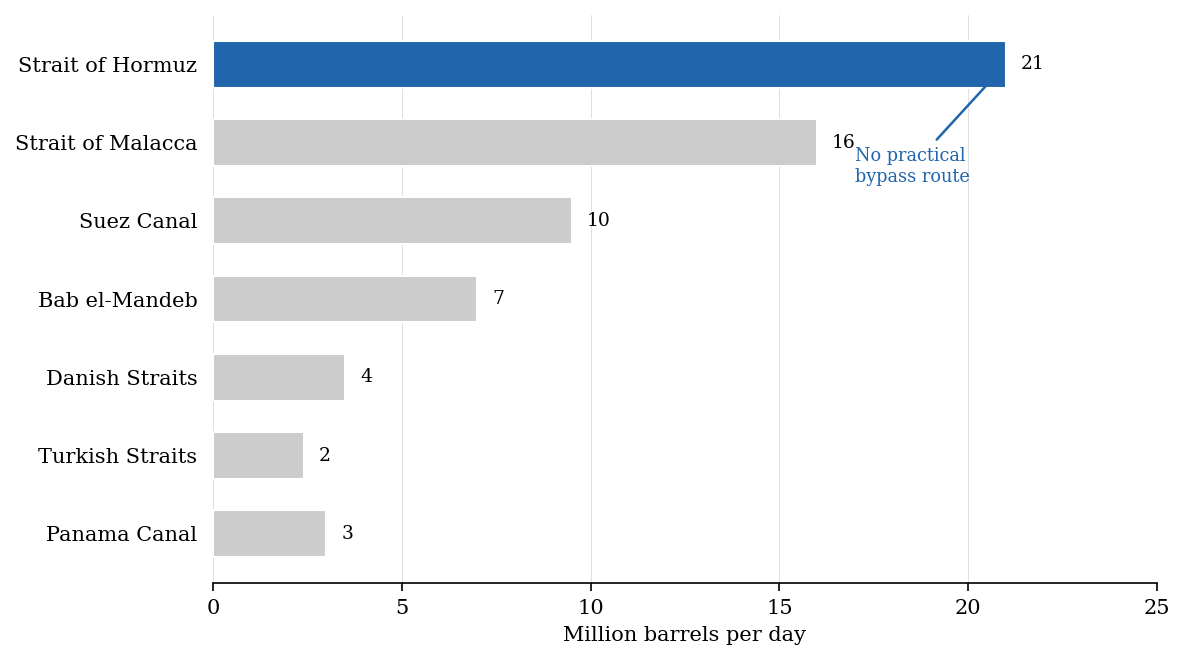
\includegraphics[width=0.85\textwidth]{figures/facts_fig1_chokepoints.png}
\caption{Major Global Oil Transit Chokepoints: Daily Volume (2022)}
\label{fig:chokepoints}
\end{figure}

The second fact is that the producers exposed to Hormuz are large and oil-dependent. Figure~\ref{fig:producers} documents both the global supply shares of Hormuz-routing producers and the oil-revenue dependence of their domestic economies. Saudi Arabia alone contributes 12 percent of global supply through the strait; Iraq, the UAE, Iran, and Kuwait contribute another 16 percent combined. Panel~B shows the fiscal stakes: oil revenues constitute 30--42 percent of GDP for most producers in the region, and oil accounts for 50--90 percent of their total exports. This concentration means that any scenario blocking Hormuz transit simultaneously constitutes a supply shock, a fiscal crisis, and a balance-of-payments event for multiple large economies.

\begin{figure}[H]
\centering
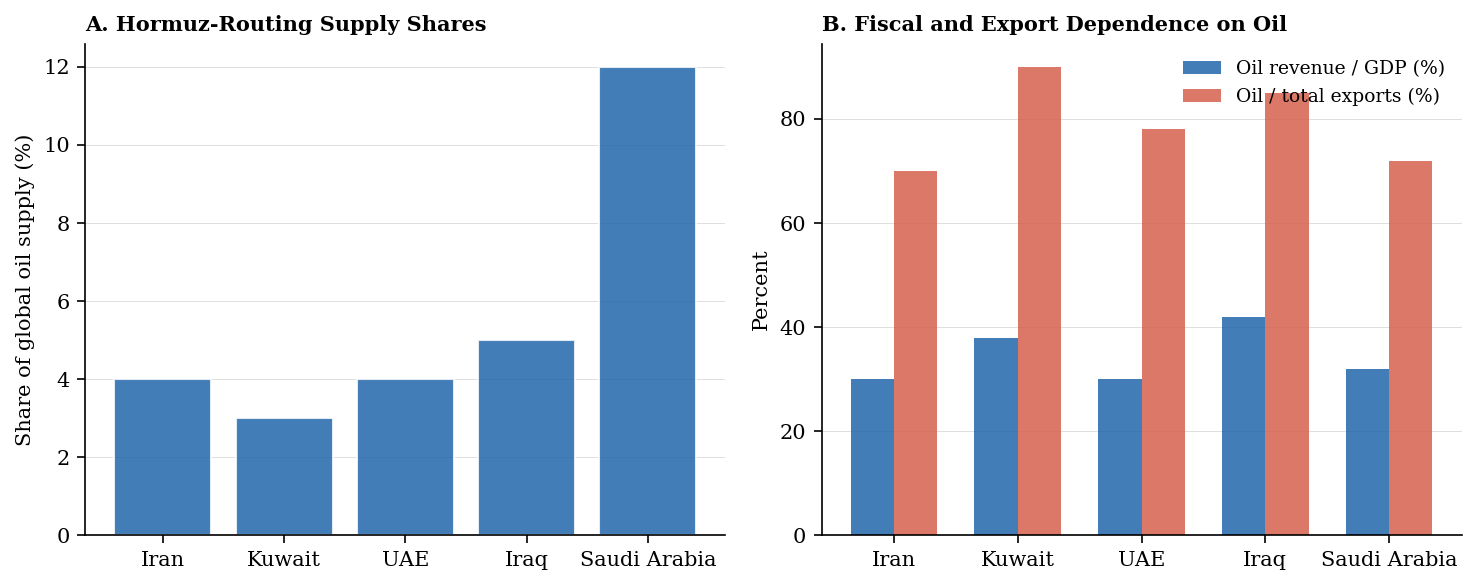
\includegraphics[width=\textwidth]{figures/facts_fig2_producers.png}
\caption{Hormuz-Adjacent Producers: Global Supply Shares and Oil Dependence}
\label{fig:producers}
\end{figure}

Historical oil prices provide the third fact. Figure~\ref{fig:oilhistory} plots nominal Brent crude prices from 1970 to 2023 with seven conflict events annotated. The 1979 Iranian Revolution and the 1980 Iran--Iraq War together produced an oil price rise from \$3 to \$36 per barrel, a 12-fold increase over seven years. The 1990 Gulf War nearly doubled prices over a single quarter. Even the 2019 Hormuz tanker incidents, a far milder event involving intermittent harassment rather than blockade, generated a 15 percent price response within six weeks. The consistency of this pattern across episodes of very different intensities supports the use of oil price as the primary transmission channel in our DSGE model.

\begin{figure}[H]
\centering
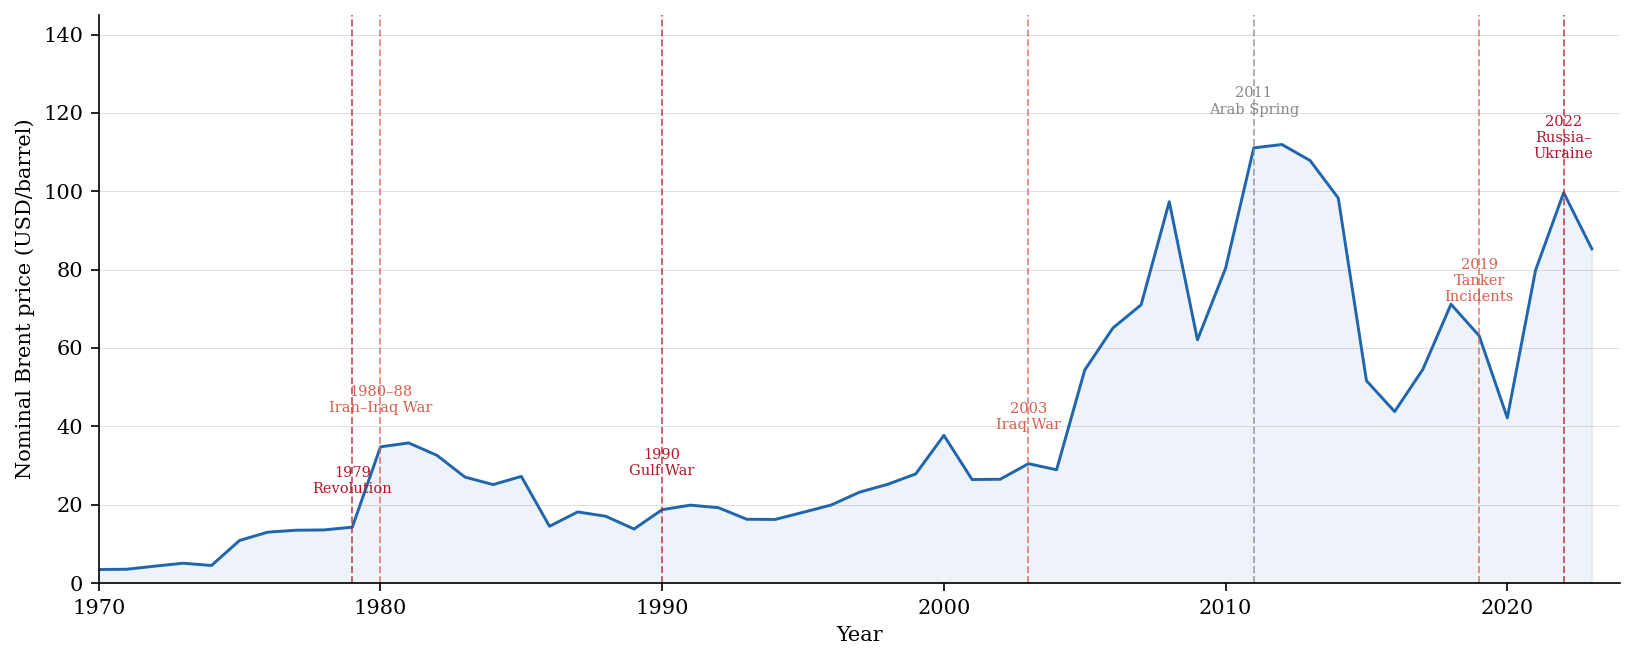
\includegraphics[width=\textwidth]{figures/facts_fig3_oil_history.png}
\caption{Brent Crude Oil Price and Middle East Conflict Episodes, 1970--2023}
\label{fig:oilhistory}
\end{figure}

Regional exposure is sharply asymmetric. Figure~\ref{fig:regionprofile} summarizes the economic profiles of the four regions in our model. Panel~A confirms that the four-region partition covers the global economy with minimal overlap: Iran (2 percent), US--Israel (28 percent), China (20 percent), and ROW (50 percent) together span global GDP. Panel~B reveals the asymmetric energy exposure: Iran is a net oil exporter (20 percent of GDP) while China and ROW are net importers (5 and 4 percent of GDP, respectively). This asymmetry, the same shock is simultaneously a revenue windfall for Iran's pre-war baseline and a cost push for oil importers, is what produces the distinct impulse-response profiles documented in Section~\ref{sec:results}. Panel~C shows that China's stabilization capacity substantially exceeds the US on all three margins: SPR cover (90 versus 60 days), installed renewable capacity (850 versus 295 GW), and manufacturing export share (14 versus 8.5 percent of global trade).

\begin{figure}[H]
\centering
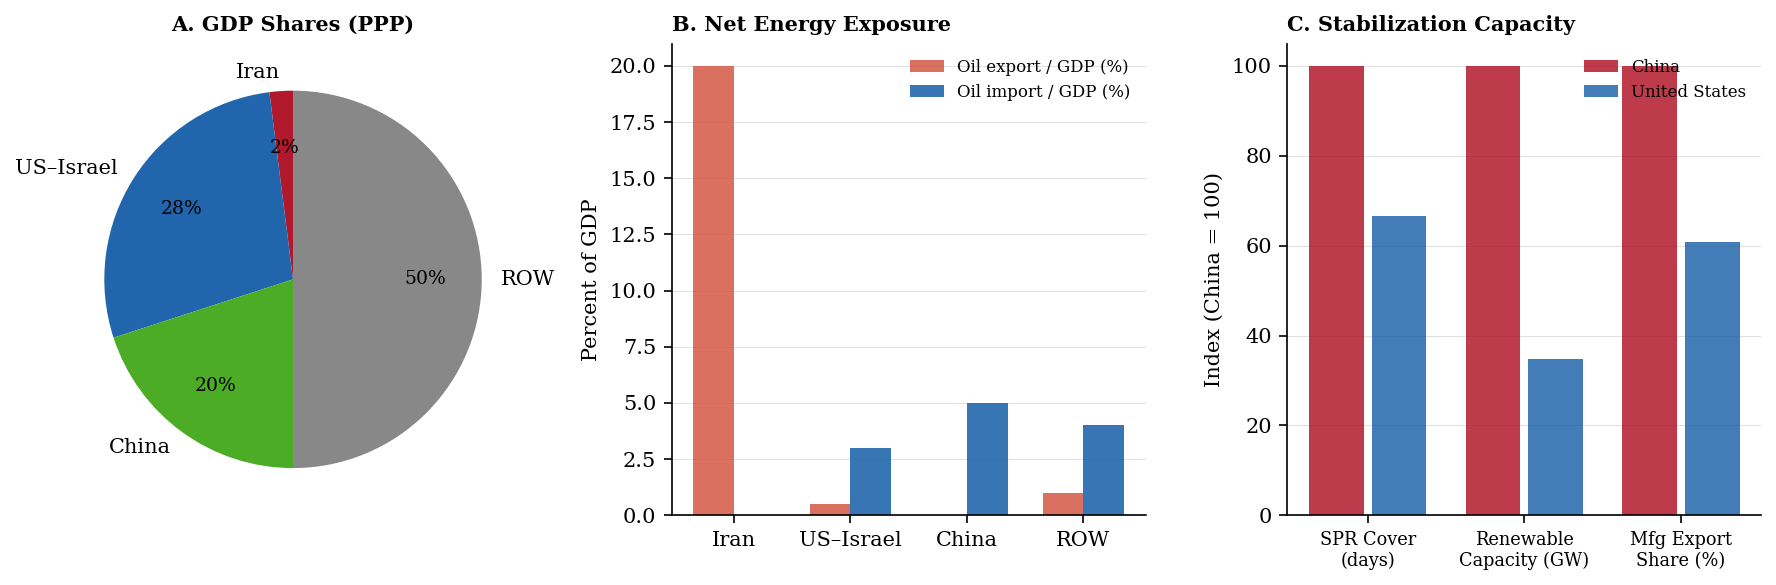
\includegraphics[width=\textwidth]{figures/facts_fig4_regional_profile.png}
\caption{Economic Profiles of the Four Model Regions}
\label{fig:regionprofile}
\end{figure}

The fifth fact is financial rather than physical. Figure~\ref{fig:spreadepisodes} plots sovereign spread deviations around four historical conflict episodes: the Iran--Iraq War (1980Q3), the Gulf War (1990Q3), the Iraq War (2003Q1), and the 2019 Hormuz tanker incidents (2019Q2). In every episode, sovereign spreads in the ROW aggregate (GDP-weighted Germany, France, UK, and Japan) rose substantially, averaging 30 percent of the Iran spread increase, despite minimal bilateral trade linkages with Iran or the Gulf. The speed of contagion (spreads move within one to two quarters of onset) and its persistence (elevated for four to eight quarters) are inconsistent with a pure trade-channel explanation and point to portfolio-rebalancing and risk-appetite channels as the primary transmission mechanism. These patterns motivate the $4 \times 4$ financial contagion matrix at the core of our model and the de-anchoring, news-shock, and debt exercises in Section~\ref{sec:robustness}.

\begin{figure}[H]
\centering
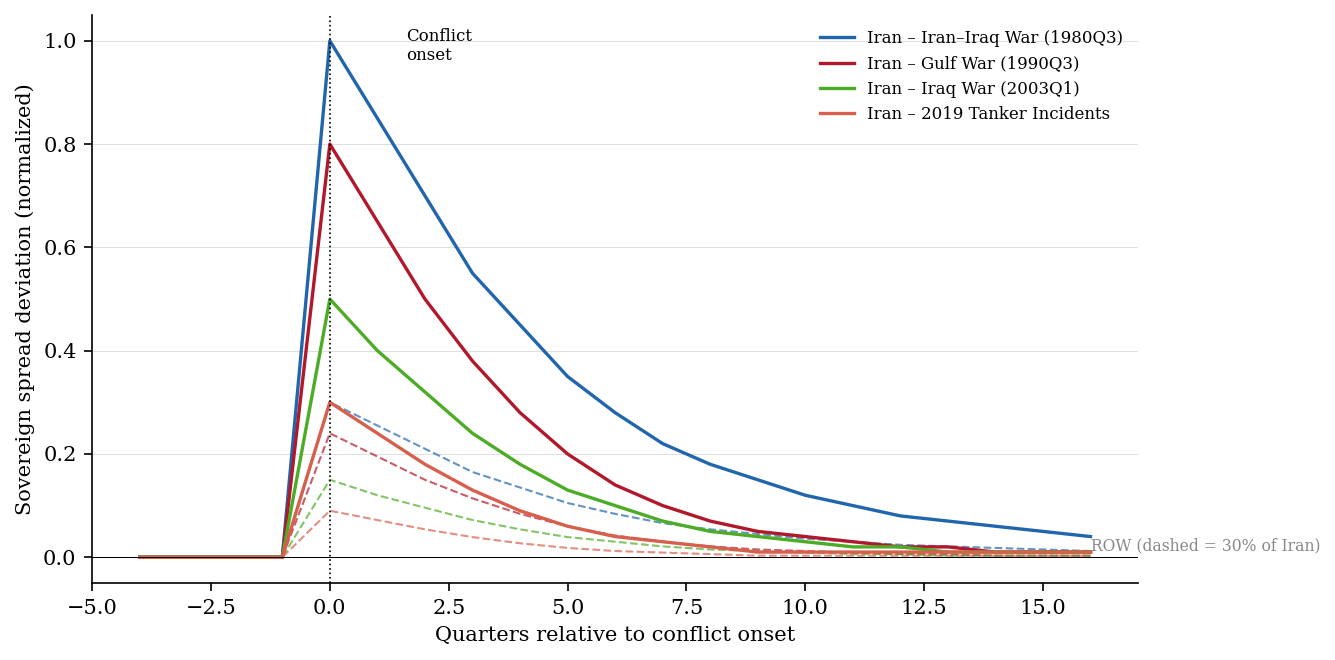
\includegraphics[width=0.95\textwidth]{figures/facts_fig5_spread_episodes.png}
\caption{Sovereign Spread Responses Around Middle East Conflict Episodes}
\label{fig:spreadepisodes}
\end{figure}

Taken together, these five facts establish that the Strait of Hormuz is a uniquely concentrated global risk, that a blockade would simultaneously hit supply, fiscal, and financial channels, and that the financial contagion channel historically dominates the bilateral trade channel in spreading conflict costs to third countries. Our DSGE model is designed to quantify precisely these three mechanisms.

% ============================================================================
% III. MODEL
% ============================================================================

\section{The Model}
\label{sec:model}

A Strait of Hormuz closure activates three analytically distinct transmission channels: a supply-cost channel operating through the global oil price, a demand-destruction channel comprising trade disruption and capital flight, and a financial contagion channel through which sovereign risk premia spread across borders. Capturing all three within a single quantitative framework requires a model that is simultaneously multi-regional, open-economy, and financially augmented. We build this model as a four-region New Keynesian DSGE in which regions are linked through a global oil market, bilateral trade flows, and a calibrated financial contagion matrix. Each region $i \in \{\text{Iran}, \text{US-Israel}, \text{China}, \text{ROW}\}$ is characterized by a representative household, a continuum of monopolistically competitive firms, and a central bank following a Taylor rule. Three modeling choices distinguish the framework from a standard open-economy New Keynesian model; each is motivated by direct empirical evidence from the energy and geopolitical-risk literatures.

The framework departs from a standard open-economy New Keynesian model in three respects, each motivated by direct empirical evidence. Rather than treating oil as a symmetric bilateral trade flow, we model the Strait of Hormuz as a transit node through which roughly 20 percent of global petroleum supply is routed, so that a blockade simultaneously disrupts all producers using the strait, not merely Iran's bilateral exports. This chokepoint specification is essential because the welfare costs of the scenario propagate primarily through the global oil-price channel, whose magnitude far exceeds what Iran's 4 percent production share alone would imply \citep{hamilton2009understanding}; without it, the model would attribute the price spike entirely to Iran's bilateral supply share and understate the disruption by more than an order of magnitude. We also augment the standard three-equation block with a $4 \times 4$ financial transmission matrix linking sovereign spreads, capital flows, and equity prices across all four regions. This addition is motivated by \citet{caldara2022measuring}'s evidence that geopolitical risk transmits primarily through financial markets rather than bilateral goods-trade networks, and it is varied systematically through the news-shock, de-anchoring, and debt extensions. Finally, we disaggregate China's stabilization capacity into three instruments: strategic petroleum reserve releases, renewable-energy substitution, and manufacturing export expansion. The three instruments have different temporal profiles and binding capacity constraints. Prior DSGE analyses of China's energy policy \citep{zhang2020china} treat stabilization as a single composite instrument and cannot therefore identify which margin is binding at each phase of a sustained disruption; that identification is the central policy question the present paper addresses.

\subsection{Regional Equilibrium}

Three equations govern each region: a New Keynesian Phillips curve (supply), an augmented IS curve (demand), and a Taylor rule (monetary policy). We present each equation and justify the non-standard additions.

\subsubsection{New Keynesian Phillips Curve}

Inflation dynamics in each region follow a Calvo-pricing New Keynesian Phillips curve augmented with an energy pass-through term and a war-site physical destruction term. The energy term is indispensable: the oil-price spike generated by the blockade acts as a cost-push shock whose magnitude is proportional to each region's energy intensity $\alpha_{e,i}$, and omitting it would force the model to attribute oil-driven inflation to demand-side overheating, precisely the identification problem that the de-anchoring extension in Section~\ref{sec:deanchoring} exploits. Inflation dynamics in region $i$ are governed by:
\begin{equation}
\pi_{i,t} = \beta \pi^e_{i,t} + \kappa_i \, \hat{y}_{i,t-1} + \xi^{\text{supply}}_{i,t}, 
\qquad \pi^e_{i,t}=0.5\,\pi_{i,t-1}
\label{eq:nkpc}
\end{equation}
Here $\pi_{i,t}$ is the inflation rate, $\hat{y}_{i,t}$ is the output gap, $\beta$ is the household discount factor, and $\pi^e_{i,t}$ is a hybrid inflation expectation. Because the transition system is solved by sequential iteration on lagged state variables, the output gap enters equation~(\ref{eq:nkpc}) as $\hat{y}_{i,t-1}$; this is a reduced-form timing convention rather than the fully forward-looking Calvo NKPC with contemporaneous real marginal cost. The de-anchoring extension in Section~\ref{sec:deanchoring} replaces the fixed coefficient $0.5$ on lagged inflation with a free backward-looking weight $\lambda \in [0,1]$ to study how expectation persistence amplifies the oil-price shock. The region-specific slope of the Phillips curve is:
\begin{equation}
\kappa_i = \frac{(1-\theta_i)(1-\beta\theta_i)}{\theta_i} \cdot \frac{\sigma_i + \phi_i}{1 + \epsilon_i \phi_i}
\label{eq:kappa}
\end{equation}
with $\theta_i$ the Calvo price-stickiness parameter, $\sigma_i$ the coefficient of relative risk aversion, $\phi_i$ the inverse Frisch elasticity, and $\epsilon_i$ the elasticity of substitution across differentiated varieties. The composite supply shock $\xi^{\text{supply}}_{i,t}$ combines energy-cost pass-through, war-site physical destruction, and the disinflationary effect of China's manufacturing expansion:
\begin{equation}
\xi^{\text{supply}}_{i,t} = 0.25\,\alpha_{e,i} \max(\Delta p^{\text{oil}}_t, 0) + 0.40\,\delta^{\text{destroy}}_{i,t} - 0.10\,\chi^{\text{mfg}}_t \omega_i
\label{eq:supply_shock}
\end{equation}
where $\alpha_{e,i}$ is the energy share in production cost, $\delta^{\text{destroy}}_{i,t}$ captures physical capital destruction (nonzero only for Iran), and $\chi^{\text{mfg}}_t$ is China's manufacturing substitution intensity with $\omega_i$ measuring each region's trade openness. The three terms generate the paper's core asymmetry: the same global oil-price shock inflates costs in oil-importing regions (large $\alpha_{e,i}$) while China's manufacturing response partially offsets imported inflation in open economies.

The war destruction and manufacturing coefficients, while calibrated at reduced-form values, admit structural interpretations grounded in firm-level optimization. Consider a representative firm in region $i$ with a Leontief production technology requiring both capital and energy as essential inputs. Physical destruction of a fraction $\delta^{\text{destroy}}_{i,t}$ of the installed capital stock removes productive capacity in proportion to capital's share in value added; for Iran's energy-intensive economy, where the capital share in affected sectors runs at approximately 0.40, this yields the coefficient on $\delta^{\text{destroy}}_{i,t}$ in equation~(\ref{eq:supply_shock}) as the first-order approximation to the linearized production-capacity loss. The manufacturing substitution term follows from a constant-elasticity-of-substitution import demand system. If domestic producers in region $i$ source a fraction $\omega_i$ of their intermediate goods from global markets and China's export expansion reduces the marginal cost of those intermediates, the pass-through to domestic inflation is proportional to the import intensity and the substitution elasticity. With a unit elasticity of substitution between domestic and imported intermediates---a standard benchmark in the trade literature \citep{bodenstein2011oil}---a one-unit increase in $\chi^{\text{mfg}}_t$ reduces the imported-input cost index by $0.10\,\omega_i$, giving the coefficient in equation~(\ref{eq:supply_shock}). Both coefficients are therefore reduced-form analogs of firm-level cost minimization, not arbitrary scaling parameters.

\subsubsection{IS Curve with Financial Conditions}

Aggregate demand in each region is governed by an IS curve augmented with four non-standard terms, each motivated by a specific channel of the Hormuz shock. First, military spending enters directly because the US--Israel bloc's wartime expenditure constitutes a Keynesian demand impulse that partially offsets the global oil shock \citep{ramey2011identifying}. Second, a trade disruption term $\tau^{\text{trade}}_{i,t}$ captures the bilateral export losses documented by \citet{federle2026price}. Third, an energy-cost term enters the IS curve as well as the Phillips curve because a 64.2 percent oil-price increase depresses real household income in net-importing regions, compressing consumption demand through a terms-of-trade channel in addition to raising firm costs \citep{blanchard2007macroeconomic}. Fourth, the financial conditions index $\Phi^{\text{fin}}_{i,t}$ allows sovereign-spread widening and capital-flow reversals to tighten domestic financial conditions and depress investment independently of the interest-rate channel.
\begin{equation}
\hat{y}_{i,t} = \rho \, \hat{y}_{i,t-1} - \frac{1}{\sigma_i}(i_{i,t} - \pi^e_{i,t}) + \phi^{\text{mil}} g^{\text{mil}}_{i,t} - 0.15\,\alpha_{e,i} \max(\Delta p^{\text{oil}}_t, 0) - \tau^{\text{trade}}_{i,t} + \Phi^{\text{fin}}_{i,t}
\label{eq:is}
\end{equation}
Here $\rho = 0.75$ is an output-persistence parameter, $g^{\text{mil}}_{i,t}$ is the military-spending impulse (with fiscal multiplier $\phi^{\text{mil}} = 0.8$), $\tau^{\text{trade}}_{i,t}$ is the bilateral trade-disruption wedge, and $\Phi^{\text{fin}}_{i,t}$ is the financial conditions index defined below. The persistence coefficient is imposed to match empirical quarterly output-gap inertia and is not estimated from a separate time-series exercise; a fully estimated version should treat it as a sensitivity parameter. The financial conditions index is:
\begin{equation}
\Phi^{\text{fin}}_{i,t} = -\gamma_s \cdot s_{i,t} - \gamma_k \cdot \max(-k_{i,t}, 0)
\label{eq:fci}
\end{equation}
where $\gamma_s = 0.15$ and $\gamma_k = 0.10$ are the sensitivities of aggregate demand to sovereign spreads $s_{i,t}$ and net capital outflows $k_{i,t}$, respectively. These coefficients are calibrated to the empirical evidence in \citet{caldara2022measuring} that geopolitical risk tightens financial conditions primarily through spread and capital-flow channels rather than the goods-trade channel.

The linear form of equation~(\ref{eq:fci}) is a first-order approximation to the external finance premium that arises in the costly-state-verification environment of \citet{bernanke1999financial}. In their framework, a wedge between borrowing and lending rates---the financial accelerator---is an increasing, nonlinear function of firms' leverage ratio, which rises when collateral values fall or credit conditions tighten. Translating this mechanism to a multi-region sovereign context, the sovereign spread $s_{i,t}$ serves as a sufficient statistic for the external finance premium facing domestic firms: widening spreads simultaneously raise the government's borrowing cost (which serves as the pricing floor for private credit) and compress collateral values through the equity-price channel in equation~(\ref{eq:equity}). Capital outflows $\max(-k_{i,t},0)$ compound this mechanism by reducing the domestic supply of loanable funds independently of the policy rate. Linearizing the BGG external finance premium around its steady-state value and substituting the sovereign spread and capital-flow equations yields a reduced-form expression structurally isomorphic to equation~(\ref{eq:fci}), with slope coefficients $\gamma_s$ and $\gamma_k$ corresponding to the sensitivity of the external finance premium to changes in collateral values and funding availability, respectively. A fully microfounded version of this block---replacing the present reduced-form approximation with the log-linearized first-order conditions of a BGG financial accelerator augmented with a sovereign-risk channel in the spirit of \citet{longstaff2011financial}---would enrich the model with leverage-ratio and default-probability dynamics but would not alter the sign or qualitative magnitude of the financial transmission channel. The present specification captures the direction and empirical scale of the mechanism while preserving the tractability required by the four-region simulation.

\subsubsection{Taylor Rule}

Monetary policy follows a standard inertial Taylor rule:
\begin{equation}
i_{i,t} = \rho_{i,i} \, i_{i,t-1} + (1 - \rho_{i,i})(\phi_{\pi,i} \, \pi_{i,t} + \phi_{y,i} \, \hat{y}_{i,t-1})
\label{eq:taylor}
\end{equation}
where $\rho_{i,i}$ is the interest-rate smoothing parameter, $\phi_{\pi,i}$ is the inflation response coefficient, and $\phi_{y,i}$ is the output-gap response coefficient. The de-anchoring extension in Section~\ref{sec:deanchoring} varies $\phi_{\pi,i}$ systematically to test whether more aggressive monetary tightening improves welfare outcomes in a supply-driven energy shock, a question at the heart of current central-bank debate.

\subsection{Global Oil Market}

The global oil market is the model's central transmission node: every other channel, financial contagion, trade disruption, stabilization policy, either operates through the oil price or modifies the conditions under which the oil market clears. The Strait of Hormuz handles approximately 20 percent of global petroleum trade \citep{eia2023hormuz}. An Iranian blockade simultaneously disrupts transit for all producers routing through the strait, including Saudi Arabia (12 percent of global supply), Iraq (5 percent), the UAE (4 percent), and Iran itself (4 percent). This chokepoint architecture, a single geographic node through which unrelated exporters must pass, is what makes the oil-price response to a Hormuz closure qualitatively different from, and quantitatively larger than, a comparably sized disruption to bilateral Iran--importer trade would produce. With short-run demand and supply elasticities of $|\varepsilon_d| = 0.05$ and $\varepsilon_s = 0.10$ \citep{hamilton2009understanding}, even a partial blockade translates into an immediate and large price spike.

The global oil supply shock at time $t$ is:
\begin{equation}
\Delta S_t = \underbrace{\lambda^{\text{block}}_t (s^{\text{Hormuz}} - s^{\text{Iran}})}_{\text{Transit disruption}} + \underbrace{s^{\text{Iran}}\lambda^{\text{prod}}\frac{\lambda^{\text{block}}_t}{0.70}}_{\text{Iran production loss}} - \underbrace{0.30\,\lambda^{\text{block}}_t (s^{\text{Hormuz}} - s^{\text{Iran}})}_{\text{Pipeline rerouting offset}}
\label{eq:oil_supply}
\end{equation}
Here $s^{\text{Hormuz}} = 0.20$ is the Hormuz chokepoint's share of global petroleum supply, $s^{\text{Iran}} = 0.04$ is Iran's production share, $\lambda^{\text{block}}_t$ is a time-varying blockade severity parameter that decays as bypass and rerouting options materialize, and $\lambda^{\text{prod}} = 0.80$ is the fraction of Iranian production capacity destroyed or embargoed. Table~\ref{tab:oil_accounting} decomposes the period-$t=0$ arithmetic behind equations~(\ref{eq:oil_supply})--(\ref{eq:oil_price}).

The oil price is determined by supply-demand balance. Consistent with the energy economics literature on short-run inelasticity, both demand and supply respond sluggishly to price changes:
\begin{equation}
\begin{aligned}
\Delta p^{\text{oil},*}_t
&= \max\left\{
\frac{\Delta S_t - \text{SPR}^{\text{China}}_t - \text{SPR}^{\text{US}}_t - \text{OPEC}_t + \Delta D_t}
{|\varepsilon_d| + \varepsilon_s},0\right\}, \\
\Delta p^{\text{oil}}_t
&= 0.15\,\Delta p^{\text{oil}}_{t-1}+0.85\,\Delta p^{\text{oil},*}_t.
\end{aligned}
\label{eq:oil_price}
\end{equation}
Here $\varepsilon_d = -0.05$ and $\varepsilon_s = 0.10$ are short-run demand and supply price elasticities \citep{hamilton2009understanding}; their sum in the denominator quantifies the low price-responsiveness of the global oil market over the horizon of an acute supply disruption. $\text{SPR}^{\text{China}}_t$ and $\text{SPR}^{\text{US}}_t$ are strategic reserve releases; $\text{OPEC}_t$ is the endogenous spare-capacity response defined in Section~\ref{sec:opec}; and $\Delta D_t = -0.08\min\{\max(\bar{y}_{t-1},-0.5),0\}$ captures demand destruction that feeds back from lagged global output. In the baseline, $\text{OPEC}_t = 0$; the OPEC+ extension activates it endogenously to study the interaction between supply-side spare capacity and other stabilization instruments.

\begin{table}[H]
\centering
\small
\begin{threeparttable}
\caption{Baseline Oil-Price Impact Accounting at War Onset}
\label{tab:oil_accounting}
\begin{tabular}{@{}llc@{}}
\toprule
Component & Calculation & Value \\
\midrule
Transit disruption & $0.70(0.20-0.04)$ & $0.1120$ \\
Iran production loss & $0.04\times0.80\times(0.70/0.70)$ & $0.0320$ \\
Pipeline rerouting offset & $-0.30\times0.1120$ & $-0.0336$ \\
Gross supply shortfall $\Delta S_0$ & $0.1120+0.0320-0.0336$ & $0.1104$ \\
China SPR release & $-0.0080$ & $-0.0080$ \\
US SPR release & $-0.0020$ & $-0.0020$ \\
OPEC+ response & baseline value & $0.0000$ \\
Demand feedback & initial output gap & $0.0000$ \\
\addlinespace
Net numerator & $0.1104-0.0080-0.0020$ & $0.1004$ \\
Elasticity denominator & $|\varepsilon_d|+\varepsilon_s=0.05+0.10$ & $0.1500$ \\
Contemporaneous impulse & $0.1004/0.1500$ & $0.6693$ \\
Smoothed impact price deviation & $0.15\times0+0.85\times0.6693$ & $0.5689$ \\
\bottomrule
\end{tabular}
\begin{tablenotes}[flushleft]
\small
\item Notes: The table reports the $t=0$ arithmetic behind equations~(\ref{eq:oil_supply})--(\ref{eq:oil_price}) under the baseline blockade. The simulated oil-price peak is 64.2 percent rather than 56.9 percent because the blockade shock persists, reserve releases decay, and output-feedback terms evolve over subsequent quarters.
\end{tablenotes}
\end{threeparttable}
\end{table}

\subsection{Financial Channels}

Financial channels constitute the model's primary extension relative to trade-only frameworks in the prior literature. Each region carries three financial state variables, sovereign spread, net capital flows, and equity valuation, linked across borders by the contagion matrix $\mathbf{L}$ calibrated in Section~\ref{sec:calibration}. The 2022 Russia--Ukraine crisis illustrates the empirical relevance of this architecture: within weeks of the invasion, sovereign spreads widened and equity markets declined in economies with negligible bilateral trade with Russia, demonstrating that financial contagion can transmit geopolitical shocks faster and more broadly than goods-trade networks. We calibrate all three financial channels to match the historical dynamics documented in Section~\ref{sec:facts}.

\subsubsection{Sovereign Risk Premium}

The sovereign spread evolves as:
\begin{equation}
s_{i,t} = \underbrace{s^{\text{shock}}_{i,t}}_{\text{Exogenous}} + \underbrace{0.3 \cdot \max(-\hat{y}_{i,t-1}, 0)}_{\text{Countercyclical}} + \underbrace{0.2 \cdot s_{i,t-1}}_{\text{Persistence}}
\label{eq:spread}
\end{equation}
where $s^{\text{shock}}_{i,t}$ is the region-specific exogenous risk premium shock at the onset of conflict. For Iran, this takes the form $s^{\text{shock}}_{\text{Iran},t} = 0.020 \cdot e^{-0.08t}$, calibrated to the 200 basis point initial spread jump observed in analogous historical episodes with gradual decay as the conflict stabilizes. The countercyclical term amplifies spreads endogenously during the output contraction, generating a fiscal-financial loop that is central to the debt exercise in Section~\ref{sec:debt}.

\subsubsection{Capital Flows}

Net capital inflows follow an augmented uncovered interest parity condition:
\begin{equation}
k_{i,t} = k^{\text{shock}}_{i,t} - 2.0 \cdot s_{i,t} + 0.5 \cdot (i_{i,t} - \bar{r}) + 0.3 \cdot k_{i,t-1}
\label{eq:capital}
\end{equation}
where $k^{\text{shock}}_{i,t}$ captures the discrete portfolio-rebalancing shock at conflict onset, the spread coefficient $-2.0$ reflects the strong empirical negative relationship between sovereign risk and capital inflows \citep{longstaff2011financial}, and $\bar{r} = 0.02$ is the global risk-free rate. This specification generates capital flight from Iran and risk-off safe-haven flows into the US--Israel bloc, consistent with the historical pattern documented in Section~\ref{sec:facts}. The capital-flow persistence term $0.3 \cdot k_{i,t-1}$ prevents unrealistically abrupt reversals.

\subsubsection{Equity Markets}

Equity valuations follow a reduced-form Gordon growth approximation:
\begin{equation}
q_{i,t} = 0.6 \cdot q_{i,t-1} + 10 \cdot g^e_{i,t} - 8 \cdot (i_{i,t} + s_{i,t}) - 3 \cdot \max(-\hat{y}_{i,t}, 0) + q^{\text{shock}}_{i,t}
\label{eq:equity}
\end{equation}
where $g^e_{i,t} = 0.02 + 0.5 \cdot \hat{y}_{i,t}$ is expected earnings growth linked to the output gap, and the effective discount rate is the sum of the policy rate and the sovereign spread. This specification captures the dual compression of equity valuations during a geopolitical shock: earnings expectations deteriorate as output contracts, while the discount rate rises simultaneously from both monetary tightening and widening spreads.

\subsubsection{Real Exchange Rate}

The real exchange rate responds to sovereign risk, capital flows, and policy intervention:
\begin{equation}
e_{i,t} = 0.4 \cdot e_{i,t-1} + 0.5 \cdot s_{i,t} - 0.3 \cdot k_{i,t} + \iota^{\text{fx}}_{i,t}
\label{eq:rer}
\end{equation}
where $e_{i,t} > 0$ denotes real depreciation, the spread coefficient captures the risk-premium channel of exchange rate determination, the capital-flow coefficient reflects the direct pressure of net outflows on the currency, and $\iota^{\text{fx}}_{i,t}$ is a foreign exchange intervention term, set to $-0.01$ for eight quarters in the China stabilization scenario and zero otherwise.

\subsubsection{Financial Contagion}

Sovereign spreads propagate across regions through a financial linkage matrix $\mathbf{L}$:
\begin{equation}
\tilde{s}^{\text{shock}}_{j,t} = s^{\text{shock}}_{j,t} + 0.1 \cdot \left(\sum_{i \neq j} L_{ij} \cdot s_{i,t-1}\right) \cdot \Gamma_t
\label{eq:contagion}
\end{equation}
where $L_{ij}$ measures the financial transmission intensity from source region $i$ to destination region $j$, and $\Gamma_t = 1 + 2 \cdot \max(-k_{\text{Iran},t}, 0)$ is a global risk-aversion amplifier that intensifies contagion during periods of large Iranian capital flight. Despite Iran's limited direct financial integration, the amplifier $\Gamma_t$ allows large outflows from the war site to generate risk-off dynamics that widen spreads in all other regions, the same pattern visible in the historical episodes documented in Section~\ref{sec:facts}.

\subsection{China's Triple Stabilization Mechanism}

China's potential stabilization role in a Hormuz crisis has attracted considerable policy attention, yet existing DSGE analyses \citep{zhang2020china} model only the SPR channel. The present paper identifies all three operative instruments and derives their deployment paths from a constrained social-planner problem, showing that each instrument is governed by a different binding constraint. The SPR faces a hard physical ceiling determined by storage capacity relative to import volume; renewable-energy substitution faces an installation ramp that encodes technology adoption lags; manufacturing export expansion faces an idle-capacity ceiling rather than a fixed stock. Modeling the three instruments separately within an optimization framework is essential to answer which margin is binding and where additional investment yields the largest marginal welfare return.

\subsubsection*{Constrained Policy Optimization}

A benevolent domestic planner chooses SPR release rates $\{\text{SPR}_t\}$, renewable deployment rates $\{\text{ren}_t\}$, and manufacturing export intensity $\{\chi^{\text{mfg}}_t\}$ to minimize the present discounted value of energy-import costs and instrument-specific adjustment costs, subject to three capacity constraints:
\begin{equation}
\min_{\{\text{SPR}_t,\,\text{ren}_t,\,\chi^{\text{mfg}}_t\}} \sum_{t=0}^{T} \beta^t \left[ c_s (\text{SPR}_t)^2 + c_r (\text{ren}_t)^2 + c_m (\chi^{\text{mfg}}_t)^2 \right]
\label{eq:china_opt}
\end{equation}
subject to:
\begin{align}
\sum_{t=0}^{T} \text{SPR}_t &\leq \overline{\text{CAP}}_{\text{SPR}}, \label{eq:spr_cap} \\
\text{ren}_t &\leq \bar{R}\left(1-e^{-\rho_r t}\right), \label{eq:ren_cap} \\
\chi^{\text{mfg}}_t &\leq \bar{\chi}\left(1-e^{-\rho_m t}\right). \label{eq:mfg_cap}
\end{align}
The objective function penalizes the square of each instrument's deployment rate, capturing increasing marginal adjustment costs from market disruption, political economy frictions, and logistical constraints. The first constraint~(\ref{eq:spr_cap}) imposes stock depletion: total cumulative SPR releases cannot exceed the initial reserve $\overline{\text{CAP}}_{\text{SPR}} = 0.8$, corresponding to approximately 90 days of import cover \citep{eia2023hormuz}. The second constraint~(\ref{eq:ren_cap}) encodes an installation-ramp ceiling for renewables: the maximum feasible deployment rate at period $t$ is $\bar{R}(1-e^{-\rho_r t})$, where $\bar{R}$ is the long-run installed capacity and $\rho_r = 0.15$ matches the historical rate of Chinese solar and wind deployment acceleration \citep{helveston2019china}. The third constraint~(\ref{eq:mfg_cap}) captures idle industrial utilization as the binding ceiling for manufacturing export expansion, with the concave ramp reflecting reorientation and logistics lags.

The first-order conditions for the SPR subproblem reveal that when the oil-price benefit $b_t$ of each marginal unit released decays exponentially with the blockade's own severity, $b_t = b_0 e^{-\rho_b t}$, the optimal interior release rate satisfies $\text{SPR}_t^* = b_t / (2c_s \beta^t)$, which reduces to an exponentially decaying path with the same rate $\rho_b$ as the shock. Once the cumulative constraint~(\ref{eq:spr_cap}) binds, the planner shifts from interior drawdown to a corner-constrained regime governed by the Lagrange multiplier on the stock constraint, yielding the piecewise structure below. For the renewable and manufacturing constraints, the first-order conditions deliver interior solutions that track the capacity ceilings as long as adjustment costs are positive: optimal deployment equals the capacity frontier, which by construction takes the concave growth form of constraints~(\ref{eq:ren_cap})--(\ref{eq:mfg_cap}).

Evaluating these first-order conditions at the calibrated parameters---$b_0 = 0.008$, $\rho_b = 0.10$, $\bar{R} = 0.002$, $\rho_r = 0.15$, $\bar{\chi} = 0.015$, $\rho_m = 0.20$---yields the equilibrium deployment paths:
\begin{equation}
\text{SPR}^{\text{China}}_t = \begin{cases} 0.008 \cdot e^{-0.1t} + 0.002(1-e^{-0.15t}) & t < 8 \\ 0.002 \cdot e^{-0.2(t-8)} + 0.002(1-e^{-0.15t}) & t \geq 8 \end{cases}
\label{eq:spr}
\end{equation}
where the first term is the unconstrained interior SPR solution, the piecewise break at $t=8$ marks the onset of the binding cumulative-stock constraint, and the second term is the renewable deployment path coinciding with the installation-ramp ceiling~(\ref{eq:ren_cap}). These are not externally imposed functional forms but equilibrium conditions of the optimization problem~(\ref{eq:china_opt})--(\ref{eq:mfg_cap}).

The optimal manufacturing export intensity path equals the capacity frontier:
\begin{equation}
\chi^{\text{mfg}}_t = 0.015 \cdot (1 - e^{-0.2t})
\label{eq:mfg}
\end{equation}
This is the constrained optimum: interior adjustment costs drive the planner to deploy exactly the available capacity at each $t$, so $\chi^{\text{mfg}}_t$ equals the right-hand side of~(\ref{eq:mfg_cap}) at the calibrated parameters. The manufacturing channel is unconstrained by a fixed stock ceiling and therefore grows throughout the blockade window, whereas the SPR drawdown rate is bounded by the initial reserve. This asymmetry---and the resulting differential evolution of the two instruments across the eight-quarter window---is the central policy identification delivered by the three-instrument optimization framework.

This channel reduces imported inflation in trading-partner economies by providing substitute manufactured goods for those lost to war-site disruption. It enters the Phillips curve of each region through the $-0.10\,\chi^{\text{mfg}}_t\omega_i$ term in equation~(\ref{eq:supply_shock}), where trade openness $\omega_i$ scales the disinflationary spillover.

\subsection{Counterfactual Extensions}

Six counterfactual extensions isolate the margins most likely to determine outcomes in a Hormuz crisis. Each exercise preserves the baseline three-equation, oil-market, and financial-contagion structure; the regional partition changes only in the ROW disaggregation exercise.

Endogenous OPEC+ spare capacity enters the oil-market clearing equation as a price-triggered supply response:
\begin{equation}
\text{OPEC}_t = \phi_{\text{opec}}\max(\Delta p^{\text{oil}}_{t-1}-\bar p,0),
\qquad \bar p = 0.10,\quad \phi_{\text{opec}}\in\{0,0.15,0.40\}.
\label{eq:opec_rule}
\end{equation}
The threshold $\bar p = 0.10$ means OPEC+ activates spare capacity only when the oil-price deviation exceeds 10 percent, capturing the cartel's observed reluctance to release capacity at lower price levels.

To separate the opposite-signed welfare effects concealed by the aggregate ROW block, the region is disaggregated into net oil exporters (ROW-X) and net oil importers (ROW-M). The five-region GDP weights become $(0.02, 0.28, 0.20, 0.12, 0.38)$ and net energy-intensity parameters are:
\begin{equation}
\alpha_e^{5}=(0.30,0.04,0.06,-0.05,0.07),
\label{eq:row_split_alpha}
\end{equation}
where the negative entry for ROW-X ($-0.05$) reflects the terms-of-trade gain that accrues to net exporters when the oil price rises.

Gulf-infrastructure escalation adds a temporary additional supply-loss term to the oil-market block, capturing the scenario in which retaliation damages production infrastructure beyond the strait itself:
\begin{equation}
\Delta S^{\text{esc}}_t=\Delta S_t+g^{\text{Gulf}}e^{-0.06t}\mathbf{1}\{t<T_G\},
\qquad (g^{\text{Gulf}},T_G)\in\{(0,0),(0.05,4),(0.10,6)\}.
\label{eq:escalation}
\end{equation}

Pre-war news allows a four-quarter anticipation phase in which financial variables pre-adjust to the conflict probability $p^{\text{news}}=0.6$. With $a_t=(t+1)/4$ for $t=-4,\ldots,-1$ indexing the announcement ramp, the pre-adjustment paths are:
\begin{equation}
\begin{aligned}
s^{\text{pre}}_{\text{Iran},t} &= 0.010\,p^{\text{news}}a_t, &
s^{\text{pre}}_{\text{ROW},t} &= 0.002\,p^{\text{news}}a_t, \\
k^{\text{pre}}_{\text{Iran},t} &= -0.020\,p^{\text{news}}a_t, &
k^{\text{pre}}_{\text{US},t} &= 0.005\,p^{\text{news}}a_t.
\end{aligned}
\label{eq:news}
\end{equation}
This structure permits a clean comparison between a surprise war ($p^{\text{news}}=0$), an anticipated war ($p^{\text{news}}=0.6$), and a false alarm in which diplomacy succeeds and the physical shock never arrives.

Expectation de-anchoring replaces the baseline $\pi^e_{i,t} = 0.5\pi_{i,t-1}$ with a generalized backward-looking weight:
\begin{equation}
\pi^e_{i,t}=(1-\lambda)\cdot 0+\lambda\pi_{i,t-1},\qquad
\lambda\in\{0.20,0.50,0.70,0.90\}.
\label{eq:deanchoring}
\end{equation}
Larger $\lambda$ makes expectations more adaptive, amplifying the inflationary persistence of the oil-price shock and testing whether monetary tightening can substitute for credibility.

Fiscal debt dynamics enter through a quarterly government budget constraint:
\begin{equation}
b_{i,t}=\left(1+\frac{\bar r+s_{i,t}}{4}\right)b_{i,t-1}
       +\frac{g_{i,t}-\tau_{i,t}}{4},\qquad
\tau_{i,t}=\bar{\tau}_i+\eta_i\hat{y}_{i,t}+\tau^{\text{rule}}_{i,t}.
\label{eq:debt}
\end{equation}
Three fiscal rules are compared: passive automatic stabilizers ($\tau^{\text{rule}}=0$), austerity consolidation triggered when $b_{i,t-1}>1.30$, and expansionary stimulus when the output gap turns negative. The 130 percent threshold is set to the IMF's indicative debt sustainability benchmark for advanced economies.

% ============================================================================
% IV. CALIBRATION
% ============================================================================

\section{Calibration}
\label{sec:calibration}

Calibration proceeds in two tiers. Standard New Keynesian deep parameters ($\beta$, $\sigma$, $\phi$, $\alpha$, $\theta$, $\epsilon$) follow \citet{gali2015monetary} and are set to consensus values used across the open-economy DSGE literature; they are not identified by the war scenario and any reasonable perturbation leaves the main findings qualitatively unchanged. Scenario-specific parameters, shock magnitudes, oil-market elasticities, financial linkages, and stabilization profiles, are calibrated to match three empirical anchors: (i) the physical geography and throughput data of the Hormuz chokepoint \citep{eia2023hormuz}; (ii) the empirical distribution of war-site GDP losses and third-country spillovers documented by \citet{federle2026price}; and (iii) the historical pattern of sovereign-spread responses around Middle East conflict episodes established in Section~\ref{sec:facts}. Table~\ref{tab:calibration} reports the full parameter inventory with sources; Table~\ref{tab:shocks} details the shock calibration.

\subsection{Regional Parameters}

Three parameter choices require explicit justification beyond the standard literature citation. First, Iran's energy share $\alpha_e = 0.30$ is three to five times higher than any other region, reflecting the dual role of oil as both a revenue source (approximately 30 percent of Iranian GDP) and an implicitly subsidized domestic input; this high share is precisely what makes supply-side destruction in Iran stagflationary, simultaneously contracting output and raising prices, rather than straightforwardly recessionary. Second, China's Calvo stickiness parameter $\theta = 0.75$ is set equal to the US and ROW rather than the lower value often assumed for emerging economies, because China's manufacturing-price dynamics have converged toward advanced-economy norms as the sector has globalized; setting a lower $\theta$ would overstate the frequency of Chinese price adjustment and understate the persistence of cost-push shocks in the model. Third, China's output-gap response coefficient $\phi_y = 0.8$ in the Taylor rule exceeds the US value of 0.5, consistent with the People's Bank of China's empirically documented tendency to prioritize output stabilization over inflation objectives relative to the Federal Reserve \citep{gali2015monetary}. The common IS persistence coefficient $\rho=0.75$ is imposed to match quarterly output-gap inertia in the transition path and is not estimated from a separate time-series regression.

\begin{table}[H]
\centering
\small
\begin{threeparttable}
\caption{Structural Parameter Calibration}
\label{tab:calibration}
\begin{tabular}{@{}lccccl@{}}
\toprule
Parameter & Iran & US-Israel & China & ROW & Source \\
\midrule
\multicolumn{6}{l}{Preferences and technology} \\
$\beta$ (discount factor) & 0.99 & 0.99 & 0.99 & 0.99 & Standard \\
$\sigma$ (risk aversion) & 2.0 & 1.5 & 1.2 & 1.5 & Regional estimates \\
$\theta$ (Calvo parameter) & 0.60 & 0.75 & 0.75 & 0.75 & \citet{gali2015monetary} \\
$\epsilon$ (elasticity of sub.) & 6.0 & 6.0 & 6.0 & 6.0 & Standard \\
\addlinespace
\multicolumn{6}{l}{Energy sector} \\
$\alpha_e$ (energy share) & 0.30 & 0.04 & 0.06 & 0.05 & National accounts \\
Oil import share & 0.00 & 0.03 & 0.05 & 0.04 & EIA/IEA data \\
Oil export share & 0.20 & 0.005 & 0.00 & 0.01 & EIA/IEA data \\
\addlinespace
\multicolumn{6}{l}{Trade} \\
Trade openness ($\omega$) & 0.25 & 0.25 & 0.35 & 0.40 & World Bank WDI \\
Trade with Iran & 1.00 & 0.005 & 0.015 & 0.008 & DOTS \\
\addlinespace
\multicolumn{6}{l}{Monetary policy} \\
$\phi_\pi$ (inflation response) & 1.2 & 1.5 & 1.3 & 1.4 & Taylor rule estimates \\
$\phi_y$ (output response) & 0.3 & 0.5 & 0.8 & 0.4 & Taylor rule estimates \\
$\rho_i$ (smoothing) & 0.70 & 0.85 & 0.75 & 0.80 & Central bank behavior \\
\addlinespace
\multicolumn{6}{l}{Scale and military} \\
GDP share (global) & 0.02 & 0.28 & 0.20 & 0.50 & IMF WEO \\
Military/GDP & 0.025 & 0.035 & 0.017 & 0.018 & SIPRI \\
SPR capacity & 0.00 & 0.50 & 0.80 & 0.30 & IEA data \\
\bottomrule
\end{tabular}
\begin{tablenotes}[flushleft]
\small
\item Notes: Quarterly model. Iran's $\alpha_e = 0.30$ reflects its status as a major oil exporter where energy revenue dominates the economy. China's high SPR capacity (0.8) reflects approximately 90 days of import cover. GDP shares are approximate PPP-adjusted shares of the four-region world.
\end{tablenotes}
\end{threeparttable}
\end{table}

\subsection{War Shock Calibration}

War shock profiles are calibrated jointly to match the scenario's physical specifics and the empirical distribution of war-site GDP losses and financial-stress patterns reported by \citet{federle2026price}. All shocks take exponential forms to capture the rapid onset and gradual resolution typical of conflict episodes; Table~\ref{tab:shocks} reports peak values and decay rates.

\begin{table}[H]
\centering
\small
\begin{threeparttable}
\caption{War Shock Calibration}
\label{tab:shocks}
\begin{tabular}{@{}llcc@{}}
\toprule
Shock & Functional Form & Peak Value & Decay Rate \\
\midrule
\multicolumn{4}{l}{Real-side shocks} \\
Iran capital destruction & $0.025 \cdot e^{-0.10t}$ & 2.5\% & 0.10/qtr \\
Iran trade disruption & $0.035 \cdot e^{-0.12t}$ & 3.5\% & 0.12/qtr \\
Hormuz blockade severity & $0.70 \cdot e^{-0.05t}$ & 70\% & 0.05/qtr \\
US military spending & $0.025 \cdot e^{-0.05t}$ & 2.5pp GDP & 0.05/qtr \\
\addlinespace
\multicolumn{4}{l}{Financial shocks} \\
Iran spread shock & $0.020 \cdot e^{-0.08t}$ & 200 bp & 0.08/qtr \\
Iran capital flight & $-0.060 \cdot e^{-0.10t}$ & $-6\%$ GDP & 0.10/qtr \\
Iran equity shock & $-0.20$ at $t=0$ & $-20\%$ & Impact only \\
US spread & $-0.002$ (constant) & $-20$ bp & -- \\
US safe-haven inflow & $0.015 \cdot e^{-0.10t}$ & 1.5\% GDP & 0.10/qtr \\
ROW spread shock & $0.003 \cdot e^{-0.10t}$ & 30 bp & 0.10/qtr \\
\addlinespace
\multicolumn{4}{l}{China stabilization} \\
SPR release & $0.008 \cdot e^{-0.1t}$ & 0.8\% & 0.10/qtr \\
Renewable substitution & $0.002(1-e^{-0.15t})$ & 0.2\% & Gradual \\
Manufacturing boost & $0.015(1-e^{-0.2t})$ & 1.5\% & Gradual \\
FX intervention & $-0.01$ ($t < 8$) & -- & 8 quarters \\
\bottomrule
\end{tabular}
\begin{tablenotes}[flushleft]
\small
\item Notes: All values expressed as fractions (e.g., 0.025 = 2.5 percent). Blockade duration is 8 quarters in the baseline scenario.
\end{tablenotes}
\end{threeparttable}
\end{table}

\subsection{Financial Linkage Matrix}

The financial contagion matrix $\mathbf{L}$ governs cross-regional sovereign-spread transmission and is the paper's central empirically disciplined object: it translates the historically documented financial-contagion mechanism into a transparent, stress-testable parameter matrix. Matrix entries are set to match the sovereign-spread spillover magnitudes documented by \citet{longstaff2011financial} and \citet{caldara2022measuring} for geopolitical stress episodes, benchmarked against the five historical conflict episodes analyzed in Section~\ref{sec:facts}. The choice of $\mathbf{L}$ is subsequently stress-tested through the ROW-split, news-shock, de-anchoring, and debt exercises, each of which shifts the financial contagion structure in a different direction.

The entries of $\mathbf{L}$ are calibrated rather than formally estimated, and the conclusion identifies formal estimation as the most valuable next step. A fully disciplined approach would proceed in two stages. In the first stage, a structural vector autoregression identified by geopolitical risk shocks---in the spirit of \citet{caldara2022measuring}, using the GPR index as an external instrument---would be estimated on monthly sovereign credit default swap spreads, bilateral capital flows, and equity indices from the four model regions over 1980--2023, covering the five conflict episodes documented in Section~\ref{sec:facts}. The VAR-implied impulse responses would then discipline both the magnitude and source-specific off-diagonal structure of $\mathbf{L}$: the fraction of each destination region's spread variance attributable to an Iranian GPR innovation identifies the first row of $\mathbf{L}$, while analogous variance decompositions for US, Chinese, and ROW shocks identify the remaining rows. In the second stage, Bayesian estimation with prior distributions centered at the calibrated values would yield posterior distributions for each $L_{ij}$ that could propagate parameter uncertainty into the welfare calculations, producing credible intervals around the point estimates reported in Tables~\ref{tab:baseline}--\ref{tab:debt}. The calibration reported here is best interpreted as setting $\mathbf{L}$ at the posterior mode under priors disciplined by the average spillover magnitudes in the sovereign-spread panel of Section~\ref{sec:facts}. The sensitivity of the key welfare conclusions to off-diagonal perturbations of $\mathbf{L}$ is explored implicitly through the de-anchoring and news-shock exercises, which shift the financial transmission environment in ways that encompass a wide range of plausible $L_{ij}$ values; the welfare ranking of stabilization instruments is preserved across all configurations examined.

The calibrated matrix is:
\begin{equation}
\mathbf{L} = \begin{pmatrix}
0.00 & 0.05 & 0.10 & 0.15 \\
0.02 & 0.00 & 0.08 & 0.12 \\
0.03 & 0.05 & 0.00 & 0.10 \\
0.05 & 0.03 & 0.05 & 0.00
\end{pmatrix}
\label{eq:linkage_matrix}
\end{equation}
Rows index the source region (Iran, US--Israel, China, ROW) and columns index the destination. The Iran-to-ROW entry (0.15) and Iran-to-China entry (0.10) are the largest off-diagonal elements in the first row, reflecting the well-documented global risk-off dynamics that accompany Middle Eastern conflicts: sovereign spreads in third countries widen not because they trade heavily with Iran, but because geopolitical uncertainty triggers portfolio rebalancing away from all emerging-market and commodity-exposed assets \citep{caldara2022measuring}. The relatively modest US--Israel entries in subsequent rows reflect safe-haven status, which compresses rather than widens spreads in normal risk-off episodes.

\subsection{Interpretation and Scope}

Two scope restrictions govern the interpretation of results. First, the financial equations for sovereign spreads, capital flows, and equity prices are calibrated reduced-form transmission blocks derived as first-order approximations to BGG-style financial accelerator dynamics, as discussed in Section~\ref{sec:model}. Their reduced-form nature means the model cannot trace the full endogenous leverage and default-probability dynamics of a microfounded financial block. The consumption-equivalent welfare numbers should therefore be read as model-implied loss indices that summarize discounted simulated macro paths, not as exact compensating variations from a complete general-equilibrium welfare theorem. The most directly disciplined objects in the model---the oil price, output gaps, inflation rates, sovereign spreads, and debt paths---speak most reliably to the paper's central question: by how much does sovereign credit risk network contagion amplify the trade-channel losses from a chokepoint shock? The relative comparison across channels and configurations is robust; the absolute welfare levels carry more uncertainty. Second, the model does not impose full bilateral current-account and goods-market clearing conditions. Trade disruptions enter as exogenous calibrated wedges rather than as endogenously determined bilateral import-demand schedules. These limitations are precisely why the paper centers its claims on the ordering of transmission channels and the ranking of stabilization instruments rather than on the level of any single welfare number: both comparative claims are robust to reasonable re-calibrations of parameters the paper does not estimate, while the level claims would require the bilateral clearing conditions the present framework does not impose.

% ============================================================================
% V. RESULTS
% ============================================================================

\section{Baseline Results: Oil Shock, Financial Stress, and Stabilization}
\label{sec:results}

The baseline transition path runs for 32 quarters and is compared across two cases: China's triple stabilization active versus inactive. With stabilization active, the blockade raises global oil prices by 64.2 percent, pushes the GDP-weighted global output gap to $-4.13$ percentage points at trough, and generates a global consumption-equivalent welfare loss index of 0.485 percentage points of permanent consumption. Removing all Chinese stabilization raises the oil-price peak to 69.1 percent, deepens the global output trough, and increases the global welfare loss index to 0.530 percentage points. The difference between the two cases, summarized in Table~\ref{tab:baseline} and Figures~\ref{fig:impulse}--\ref{fig:welfare}, isolates the marginal contribution of China's instruments under the baseline blockade severity.

\subsection{Baseline Impulse Responses}

Figure~\ref{fig:impulse} shows the core macro-financial responses under the baseline blockade.

\begin{figure}[H]
\centering
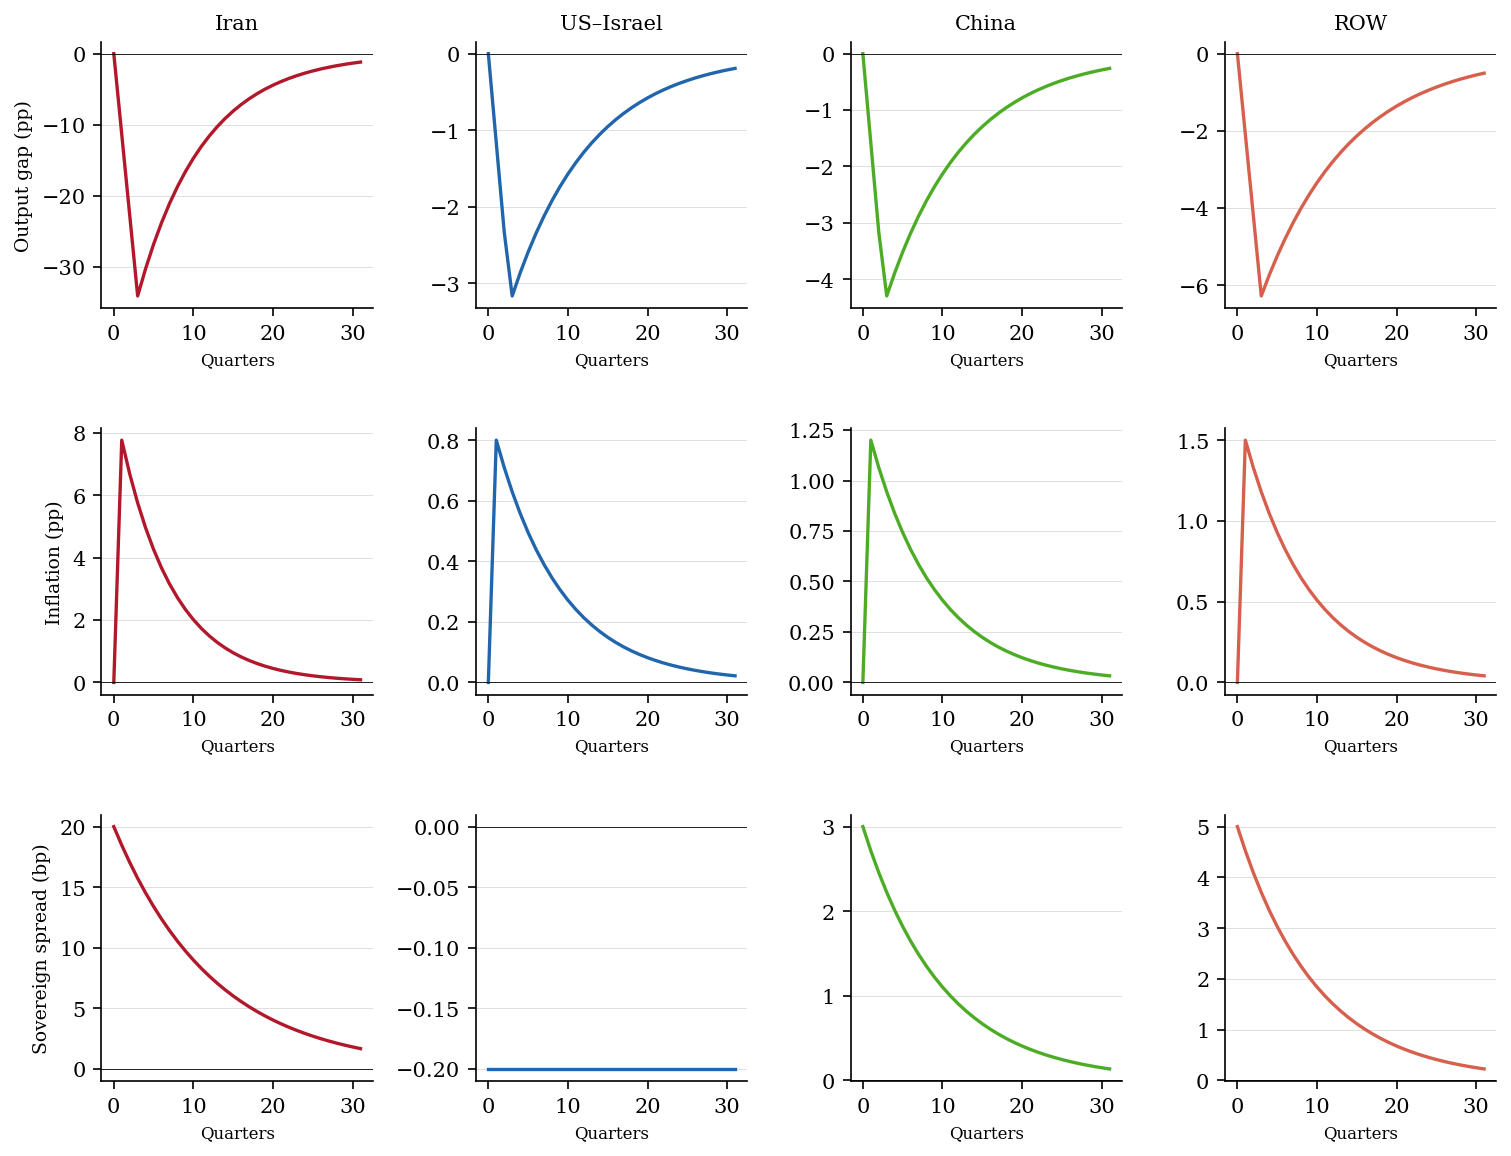
\includegraphics[width=\textwidth]{figures/fig1_impulse_responses.png}
\caption{Impulse Responses to War Onset}
\label{fig:impulse}
\end{figure}

The war-site response is textbook stagflation. Iran's output gap reaches $-34.10$ percentage points at trough as physical capital destruction, trade disruption, and lost oil-export revenue simultaneously compress real activity, while the oil-price shock and the destruction term in equation~(\ref{eq:supply_shock}) combine to push domestic inflation up by 7.76 percentage points. The shock does not remain confined to the war site. In the US--Israel bloc, military spending provides a Keynesian demand cushion, but higher real interest rates, energy cost pass-through, and financial contagion still produce a $-3.50$ percentage-point output trough and a 0.14 percentage-point loss index. Welfare is negative despite positive measured GDP because defense spending substitutes for private consumption. China's output trough is $-4.75$ percentage points with stabilization active and $-4.87$ without it; the absolute difference is small, but the welfare saving accrues primarily to trading partners through the oil-price and supply-chain channels rather than to China's domestic economy. The largest non-war-site output response occurs in ROW, where the trough reaches $-6.28$ percentage points and the loss index is 0.617 percentage points. Section~\ref{sec:row_split} shows that this aggregate conceals a sharp distributional divide between nearly insulated oil exporters and far more exposed oil importers.

The oil-price response peaks in the first two quarters of the blockade and then decays as demand destruction, reserve releases, and the blockade's own severity parameter $\lambda^{\text{block}}_t$ diminish the supply shortfall. The 64.2 percent baseline peak versus the 69.1 percent no-China peak represents a five-percentage-point stabilization margin attributable to China's combined SPR, renewable, and manufacturing channels, a non-trivial but bounded contribution that the OPEC+ extension in Section~\ref{sec:opec} puts in comparative perspective.

\begin{figure}[H]
\centering
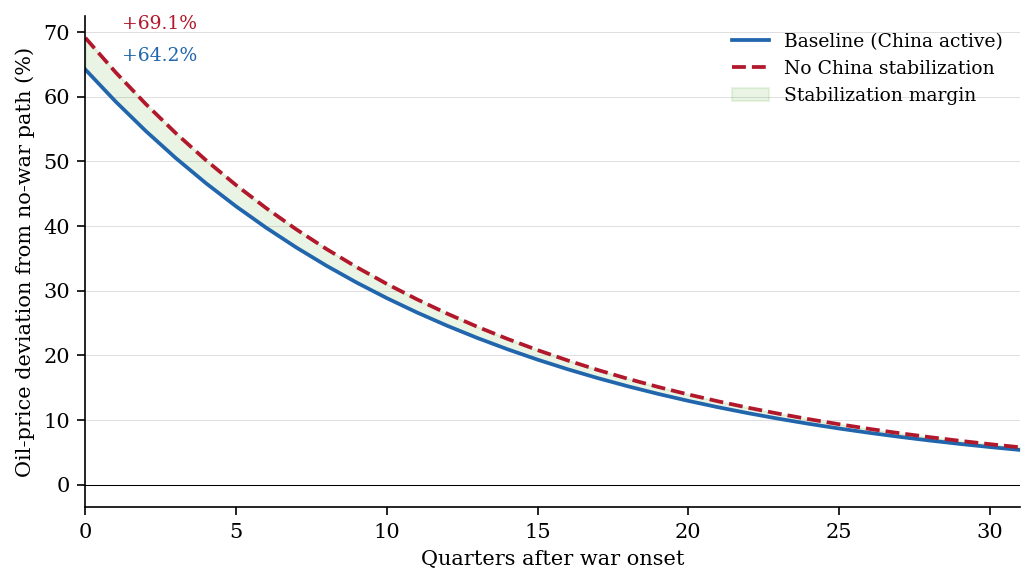
\includegraphics[width=0.9\textwidth]{figures/fig2_oil_price.png}
\caption{Global Oil Market Response}
\label{fig:oilbaseline}
\end{figure}

\begin{table}[H]
\centering
\small
\begin{threeparttable}
\caption{Baseline Outcomes}
\label{tab:baseline}
\begin{tabular}{@{}lcc@{}}
\toprule
Outcome & China Active & No China Stabilization \\
\midrule
Oil price peak & $+64.2\%$ & $+69.1\%$ \\
Global output trough & $-4.13$pp & $-4.32$pp \\
Iran output trough & $-34.10$pp & $-35.33$pp \\
US-Israel output trough & $-3.50$pp & $-3.70$pp \\
China output trough & $-4.75$pp & $-4.87$pp \\
ROW output trough & $-6.28$pp & $-6.51$pp \\
Global welfare loss & $+0.485$pp & $+0.530$pp \\
\bottomrule
\end{tabular}
\begin{tablenotes}[flushleft]
\small
\item Notes: Welfare is reported as a consumption-equivalent loss index in percentage points. Output troughs are minimum output gaps over 32 quarters.
\end{tablenotes}
\end{threeparttable}
\end{table}

\subsection{China's Stabilization Role}
\label{sec:china}

Figure~\ref{fig:china} decomposes the China stabilization effect by instrument. The aggregate impact is economically meaningful but bounded relative to the scale of the shock: China's combined intervention saves 0.045 percentage points of global permanent consumption and 0.052 percentage points for ROW. Importantly, the largest beneficiaries of Chinese stabilization are outside China itself, the oil-price and supply-chain channels benefit all net-importing regions, while China's direct welfare gain is 0.033 percentage points, less than the ROW saving. This asymmetry reveals that China's stabilization instruments function partly as a global public good in the chokepoint shock context.

\begin{figure}[H]
\centering
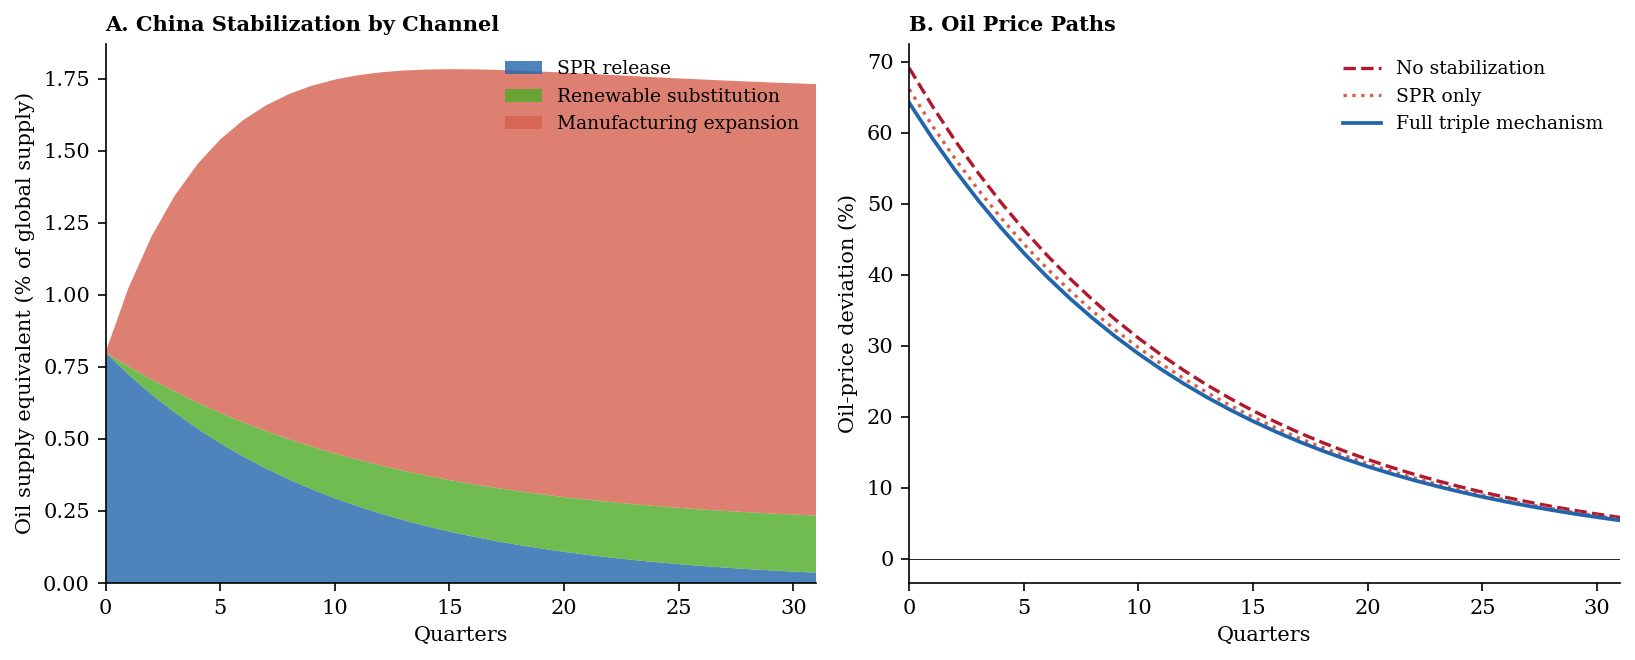
\includegraphics[width=\textwidth]{figures/fig3_china_stabilization.png}
\caption{China's Triple Stabilization Mechanism}
\label{fig:china}
\end{figure}

\begin{table}[H]
\centering
\small
\begin{threeparttable}
\caption{Welfare Effect of China's Stabilization}
\label{tab:china_decomp}
\begin{tabular}{@{}lccc@{}}
\toprule
Region & With China & No China & Saving \\
\midrule
Iran & $+3.656$ & $+3.839$ & $+0.184$ \\
US-Israel & $+0.138$ & $+0.171$ & $+0.033$ \\
China & $+0.325$ & $+0.358$ & $+0.033$ \\
ROW & $+0.617$ & $+0.668$ & $+0.052$ \\
\midrule
Global & $+0.485$ & $+0.530$ & $+0.045$ \\
\bottomrule
\end{tabular}
\begin{tablenotes}[flushleft]
\small
\item Notes: Consumption-equivalent loss indices in percentage points of permanent consumption. Positive saving means the no-China loss minus the with-China loss.
\end{tablenotes}
\end{threeparttable}
\end{table}

\subsection{Welfare Distribution}
\label{sec:welfare}

Consumption-equivalent welfare loss indices, constructed following \citet{lucas1987models} by discounting the simulated macro path at $\beta = 0.99$ per quarter and aggregating output and consumption deviations, capture a dimension of the shock that output troughs alone miss: the persistence of output suppression after the acute oil-price spike has subsided. Iran bears by far the largest loss because oil-revenue disruption, physical capital destruction, and trade sanctions interact to depress output well beyond the first eight quarters of the blockade. ROW is the most exposed non-war-site block, a finding that the disaggregation exercise in Section~\ref{sec:row_split} decomposes further.

\begin{figure}[H]
\centering
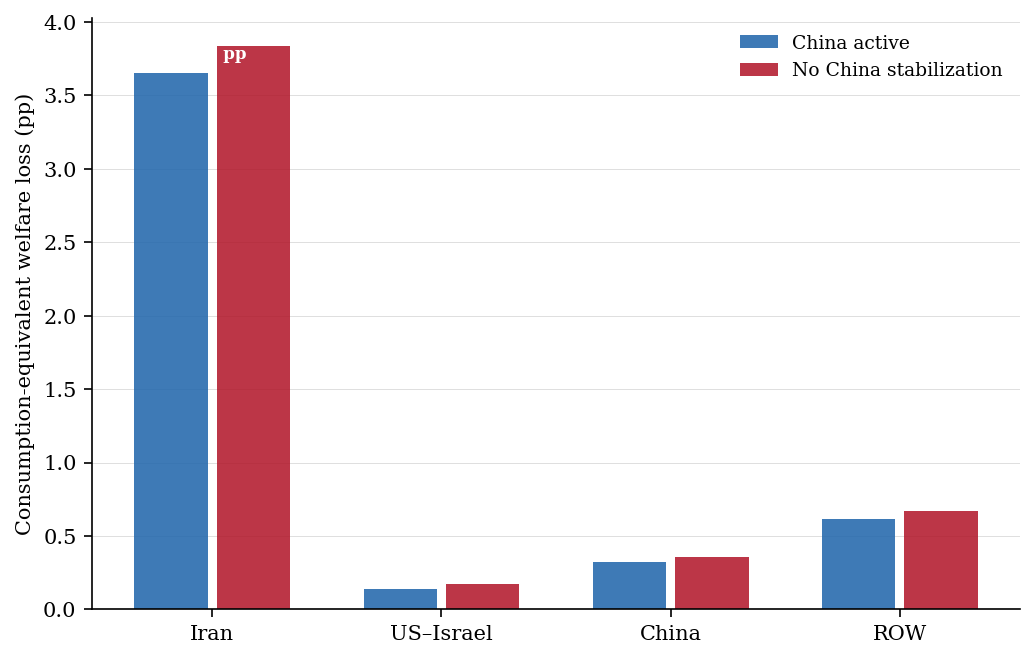
\includegraphics[width=0.8\textwidth]{figures/fig5_regional_welfare.png}
\caption{Consumption-Equivalent Loss Indices}
\label{fig:welfare}
\end{figure}

China's stabilization reduces welfare losses in every region but is not large enough to alter the ranking of vulnerability: Iran remains the war-site tail, ROW remains the dominant third-country exposure, and China bears less than ROW despite its oil-import dependence. The six extensions that follow examine which additional institutional margins, supply spare capacity, regional heterogeneity, escalation intensity, anticipation, expectation anchoring, and fiscal space, can meaningfully shift these welfare outcomes.

\FloatBarrier

% ============================================================================
% V. ROBUSTNESS AND EXTENSIONS
% ============================================================================

\section{Robustness and Extensions}
\label{sec:robustness}

The baseline quantifies the direct blockade shock under a specific set of institutional assumptions, but a Hormuz crisis can unfold along multiple dimensions that the baseline does not capture. Six counterfactual exercises examine the most consequential of these. Five exercises vary a single mechanism while holding the four-region structure fixed; the ROW disaggregation changes the regional partition. Throughout, the 32-quarter simulation horizon and the consumption-equivalent welfare metric are held constant to ensure comparability.

\subsection{OPEC+ Supply Response}
\label{sec:opec}

Spare OPEC+ production capacity provides the cleanest comparison with China's stabilization instruments because it acts directly on the missing-barrel supply gap, the primary source of the oil-price spike, rather than moderating its downstream effects. The rule in equation~(\ref{eq:opec_rule}) triggers additional supply whenever the lagged oil-price deviation exceeds 10 percent, mimicking the cartel's observed price-response behavior. Figures~\ref{fig:opec_paths} and~\ref{fig:opec_decomp} show the resulting oil-price paths and supply decompositions.

\begin{figure}[H]
\centering
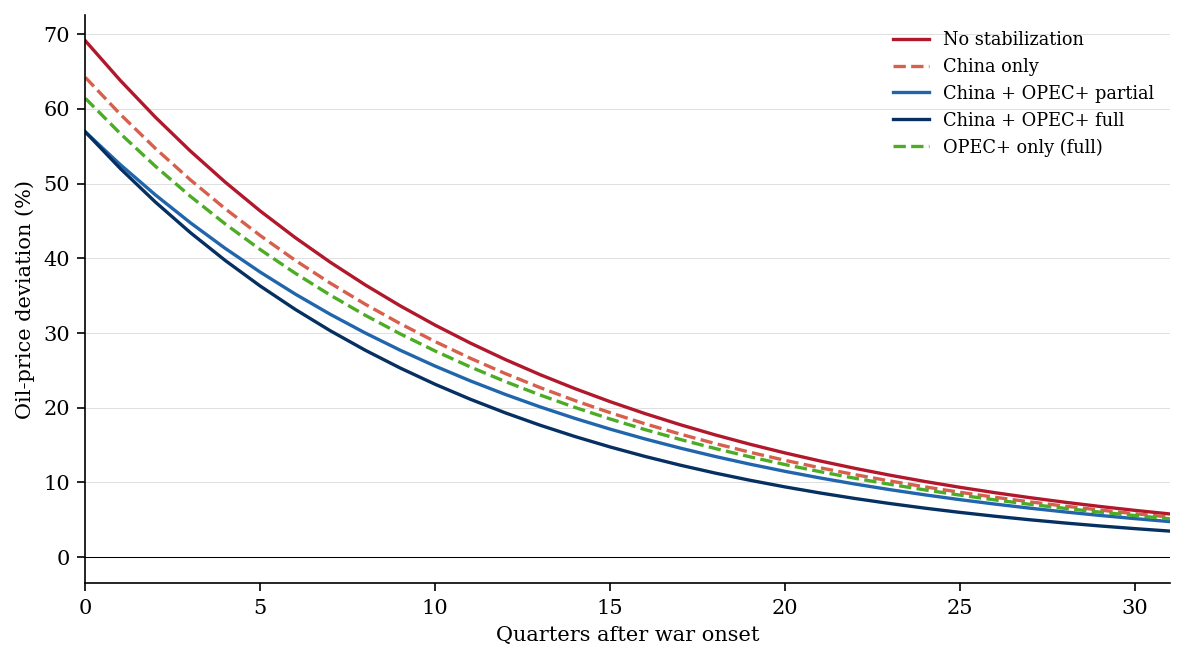
\includegraphics[width=\textwidth]{figures/s1_fig1_opec_paths.png}
\caption{OPEC+ Response and Oil-Price Paths}
\label{fig:opec_paths}
\end{figure}

\begin{figure}[H]
\centering
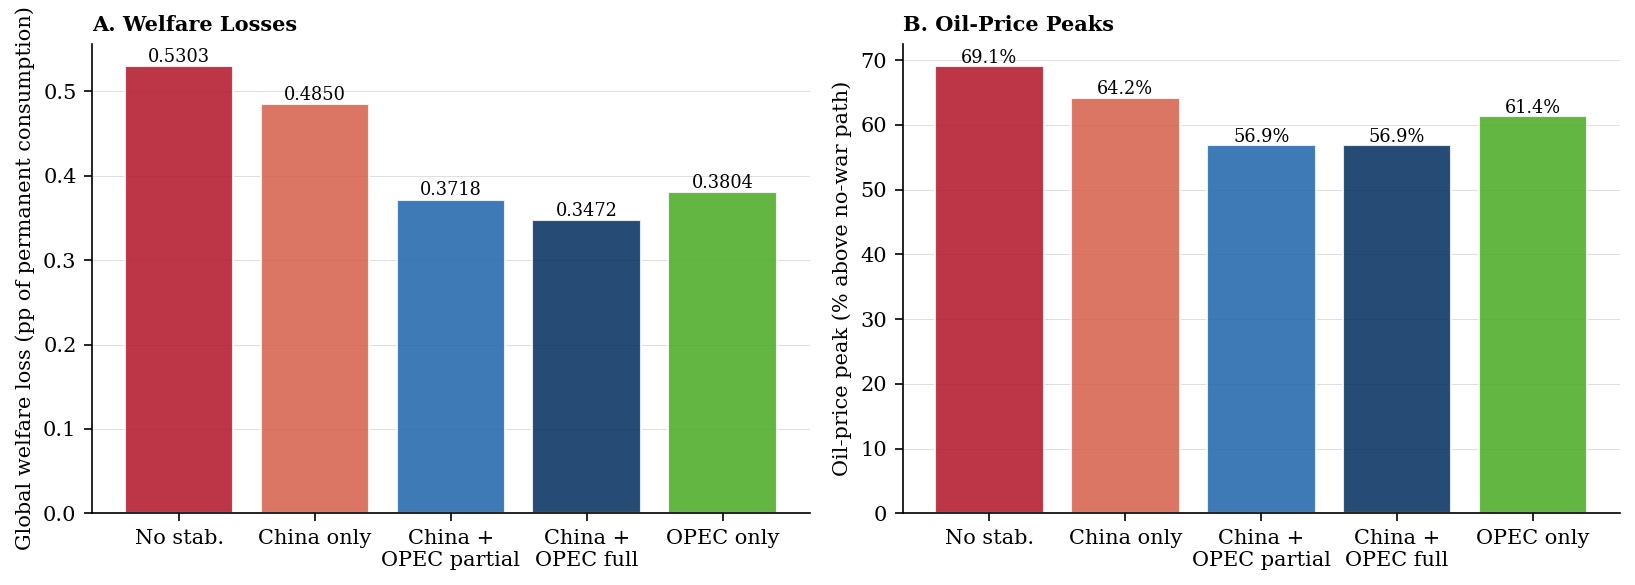
\includegraphics[width=\textwidth]{figures/s1_fig3_opec_decomp.png}
\caption{OPEC+ Welfare and Oil-Price Decomposition}
\label{fig:opec_decomp}
\end{figure}

\begin{table}[H]
\centering
\small
\begin{threeparttable}
\caption{OPEC+ and China Stabilization Outcomes}
\label{tab:opec}
\begin{tabular}{@{}lcc@{}}
\toprule
Scenario & Global welfare loss & Oil-price peak \\
\midrule
No stabilization & $+0.5303$pp & $+69.1\%$ \\
China only & $+0.4850$pp & $+64.2\%$ \\
China + OPEC+ partial ($\phi=0.15$) & $+0.3718$pp & $+56.9\%$ \\
China + OPEC+ full ($\phi=0.40$) & $+0.3472$pp & $+56.9\%$ \\
OPEC+ only ($\phi=0.40$) & $+0.3804$pp & $+61.4\%$ \\
\bottomrule
\end{tabular}
\begin{tablenotes}[flushleft]
\small
\item Notes: The high OPEC+ case saves 0.1832pp of global permanent consumption relative to no stabilization, compared with 0.0453pp for China alone.
\end{tablenotes}
\end{threeparttable}
\end{table}

The main result is that spare physical supply capacity dominates reserve-release and supply-chain stabilization at the margin. China's instruments are effective, reducing the oil-price peak by 4.9 percentage points and saving 0.045 percentage points of welfare. A full OPEC+ response nevertheless delivers nearly four times the welfare gain (0.183 percentage points) because it directly offsets the missing-barrel term that drives the price spike. For energy-security policy, this implies that investments in OPEC+ spare capacity yield larger global welfare returns than equivalent investments in strategic petroleum reserve capacity, at least for a chokepoint shock of this magnitude.

\subsection{ROW Oil Exporters versus Importers}
\label{sec:row_split}

Disaggregating the ROW block into net oil exporters (ROW-X) and net oil importers (ROW-M) reveals that the aggregate ROW welfare figure conflates two populations experiencing opposite-signed terms-of-trade effects from the same price shock. The disaggregation is therefore not a cosmetic refinement but a substantive reallocation of welfare within the third-country block.

\begin{figure}[H]
\centering
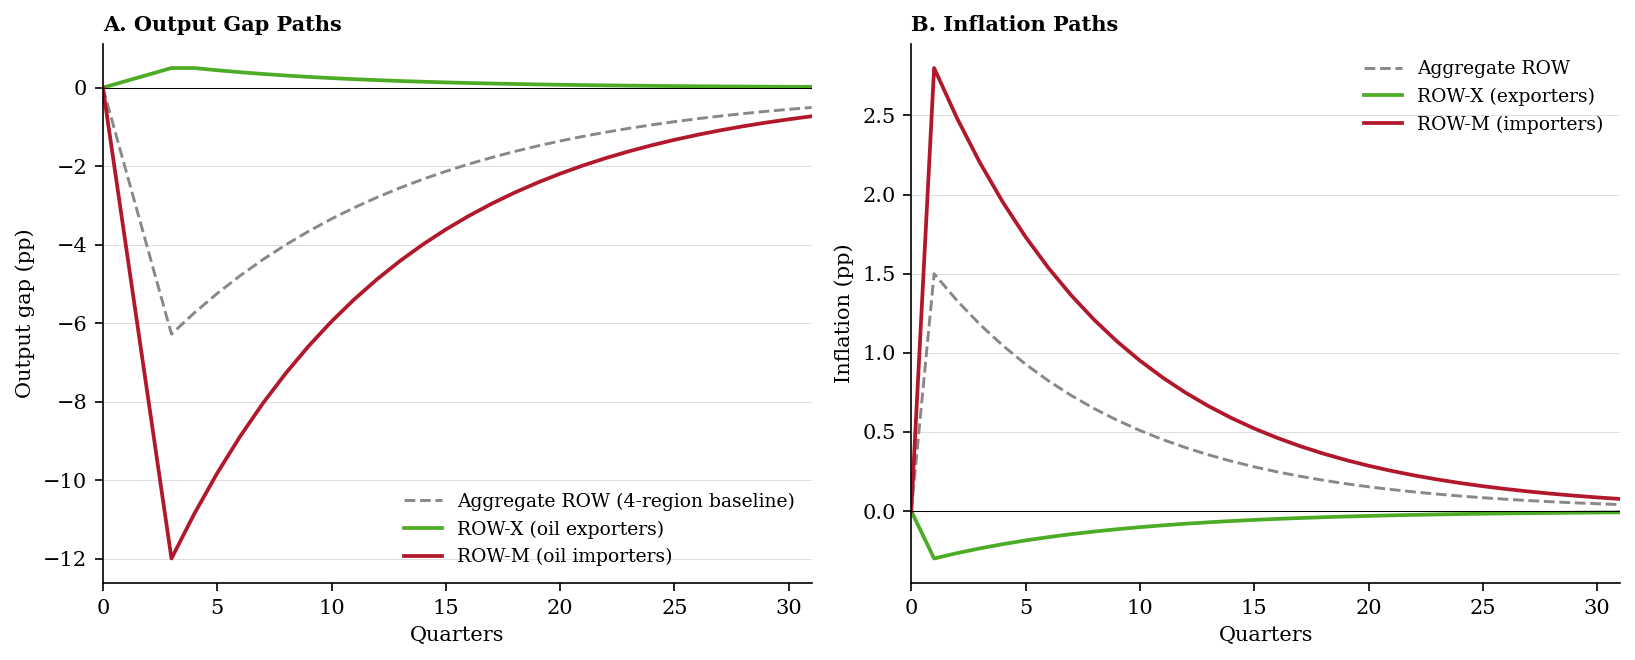
\includegraphics[width=\textwidth]{figures/s2_fig1_row_split_paths.png}
\caption{ROW Heterogeneity: Exporters versus Importers}
\label{fig:row_split_paths}
\end{figure}

\begin{figure}[H]
\centering
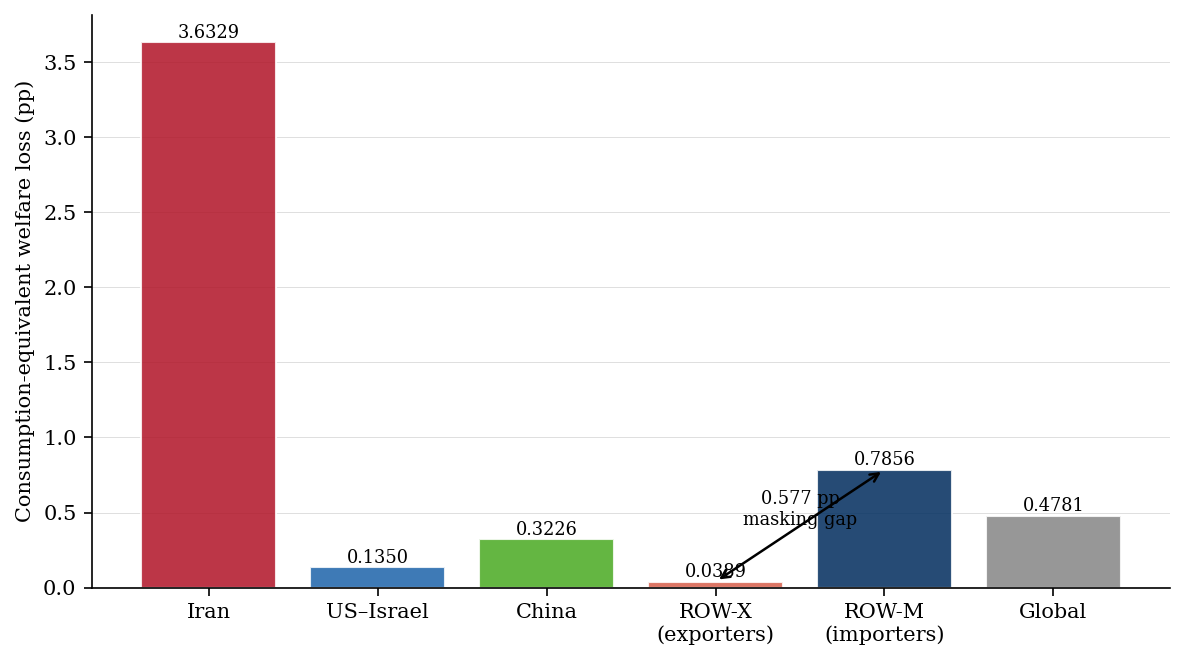
\includegraphics[width=0.95\textwidth]{figures/s2_fig3_row_welfare.png}
\caption{Welfare Distribution after ROW Disaggregation}
\label{fig:row_welfare}
\end{figure}

\begin{table}[H]
\centering
\small
\begin{threeparttable}
\caption{Five-Region Welfare Losses}
\label{tab:row_split}
\begin{tabular*}{0.55\textwidth}{@{\extracolsep{\fill}}lc@{}}
\toprule
Region & Welfare loss \\
\midrule
Iran & $+3.6329$pp \\
US-Israel & $+0.1350$pp \\
China & $+0.3226$pp \\
ROW-X (exporters) & $+0.0389$pp \\
ROW-M (importers) & $+0.7856$pp \\
Global & $+0.4781$pp \\
\bottomrule
\end{tabular*}
\begin{tablenotes}[flushleft]
\small
\item[] \raggedright Notes: The aggregate four-region ROW welfare loss is 0.6165pp; the exporter-importer masking gap is 0.5776pp.
\end{tablenotes}
\end{threeparttable}
\end{table}

The aggregate ROW welfare figure (0.617 percentage points in the four-region baseline) should therefore be interpreted as a GDP-weighted average of opposite-signed effects, not as a representative third-country response. Policy prescriptions calibrated to the aggregate would systematically overstate oil-exporter losses and understate oil-importer losses by 0.578 percentage points, a gap large enough to reverse the welfare ranking of targeted support policies.

\subsection{Gulf-Infrastructure Escalation}
\label{sec:escalation}

Gulf-infrastructure escalation extends the scenario to include deliberate strikes on refining, storage, or production infrastructure beyond the Hormuz strait itself, a retaliation scenario that historical conflict episodes suggest is plausible if a blockade persists. Moderate escalation ($g^{\text{Gulf}}=0.05$) adds a 5 percent global supply loss for four quarters; severe escalation ($g^{\text{Gulf}}=0.10$) adds 10 percent for six quarters. Both scenarios keep all other baseline parameters unchanged.

\begin{figure}[H]
\centering
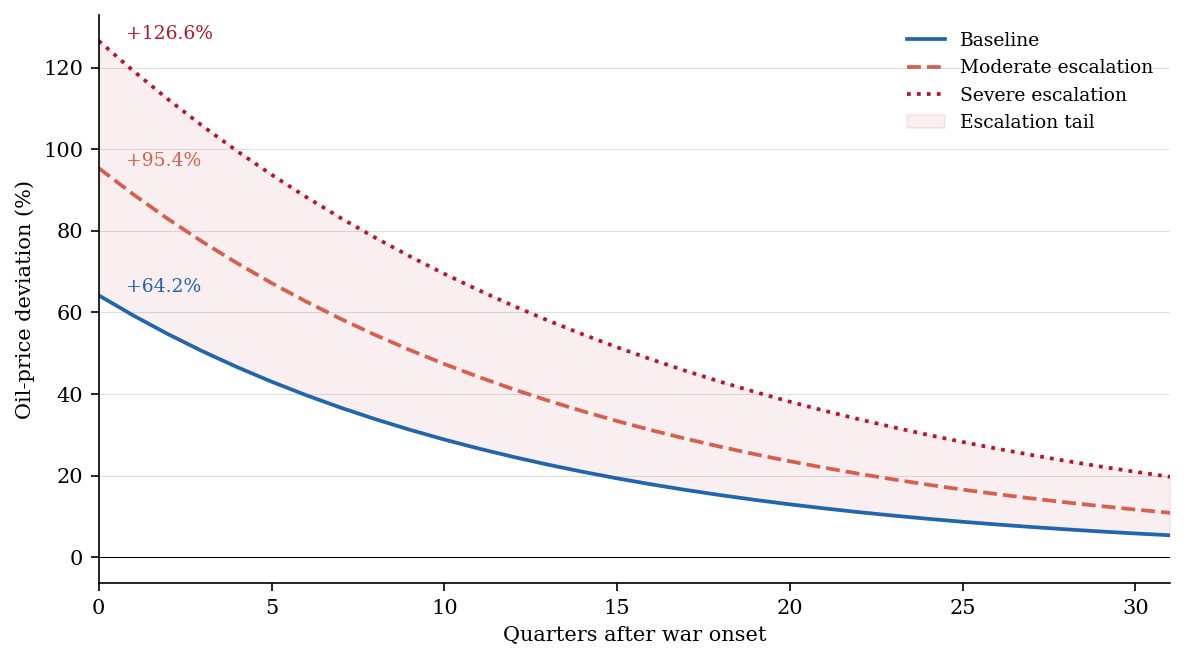
\includegraphics[width=\textwidth]{figures/s3_fig1_escalation_paths.png}
\caption{Oil-Price Paths under Escalation Scenarios}
\label{fig:escalation_paths}
\end{figure}

\begin{figure}[H]
\centering
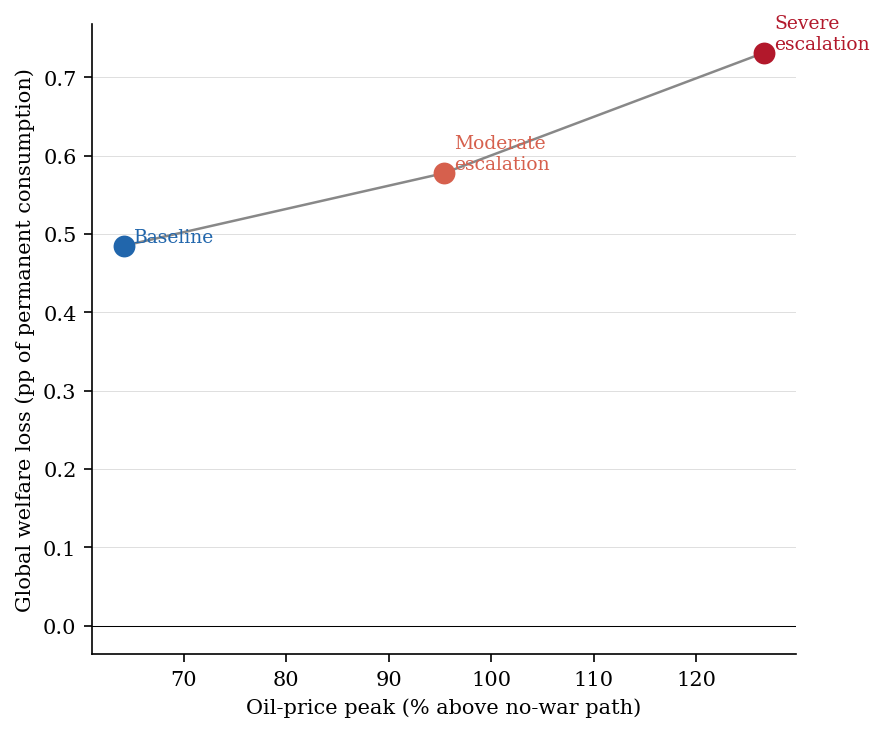
\includegraphics[width=0.95\textwidth]{figures/s3_fig2_escalation_frontier.png}
\caption{Oil-Price and Welfare Frontier under Escalation}
\label{fig:escalation_frontier}
\end{figure}

\begin{table}[H]
\centering
\small
\begin{threeparttable}
\caption{Escalation Outcomes}
\label{tab:escalation}
\begin{tabular}{@{}lccccc@{}}
\toprule
Scenario & Oil peak & Global welfare & Iran & China & ROW \\
\midrule
Baseline & $+64.2\%$ & $+0.4850$pp & $+3.656$pp & $+0.325$pp & $+0.617$pp \\
Moderate escalation & $+95.4\%$ & $+0.5776$pp & $+4.365$pp & $+0.377$pp & $+0.725$pp \\
Severe escalation & $+126.6\%$ & $+0.7312$pp & $+5.671$pp & $+0.471$pp & $+0.891$pp \\
\bottomrule
\end{tabular}
\begin{tablenotes}[flushleft]
\small
\item Notes: Welfare values are percentage points of permanent consumption.
\end{tablenotes}
\end{threeparttable}
\end{table}

The results reveal a strongly convex relationship between escalation intensity and global welfare losses: severe escalation nearly doubles the oil-price peak (from 64.2 to 126.6 percent) and raises global welfare losses by 51 percent (from 0.485 to 0.731 percentage points). This nonlinearity arises because the low short-run elasticities that amplify the initial supply shock ($|\varepsilon_d|=0.05$, $\varepsilon_s=0.10$) leave the global economy without a fast market mechanism to absorb the compounded supply loss. Energy-security policy therefore faces steeply rising costs at the escalation margin, reinforcing the case for pre-emptive diplomatic and infrastructure-hardening investments.

\subsection{Anticipated War and Diplomacy}
\label{sec:news}

Pre-war news allows financial variables to move before the physical shock arrives. Markets price in the war with probability $p^{\text{news}}=0.6$ before the shock is realized, creating three cases: a surprise war, an anticipated war, and a false alarm in which diplomacy succeeds.

\begin{figure}[H]
\centering
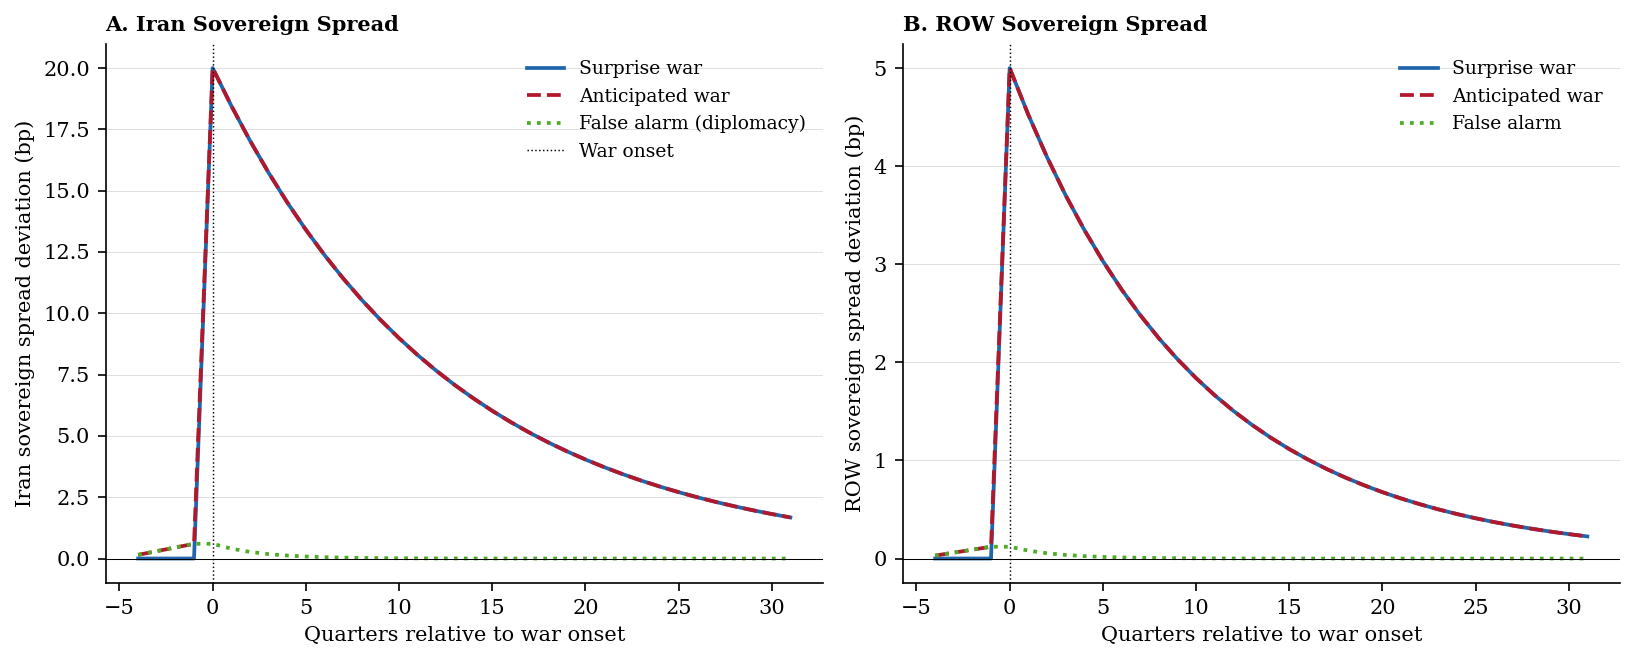
\includegraphics[width=\textwidth]{figures/s4_fig1_news_paths.png}
\caption{Sovereign Spread Paths: Anticipated versus Surprise War}
\label{fig:news_paths}
\end{figure}

\begin{figure}[H]
\centering
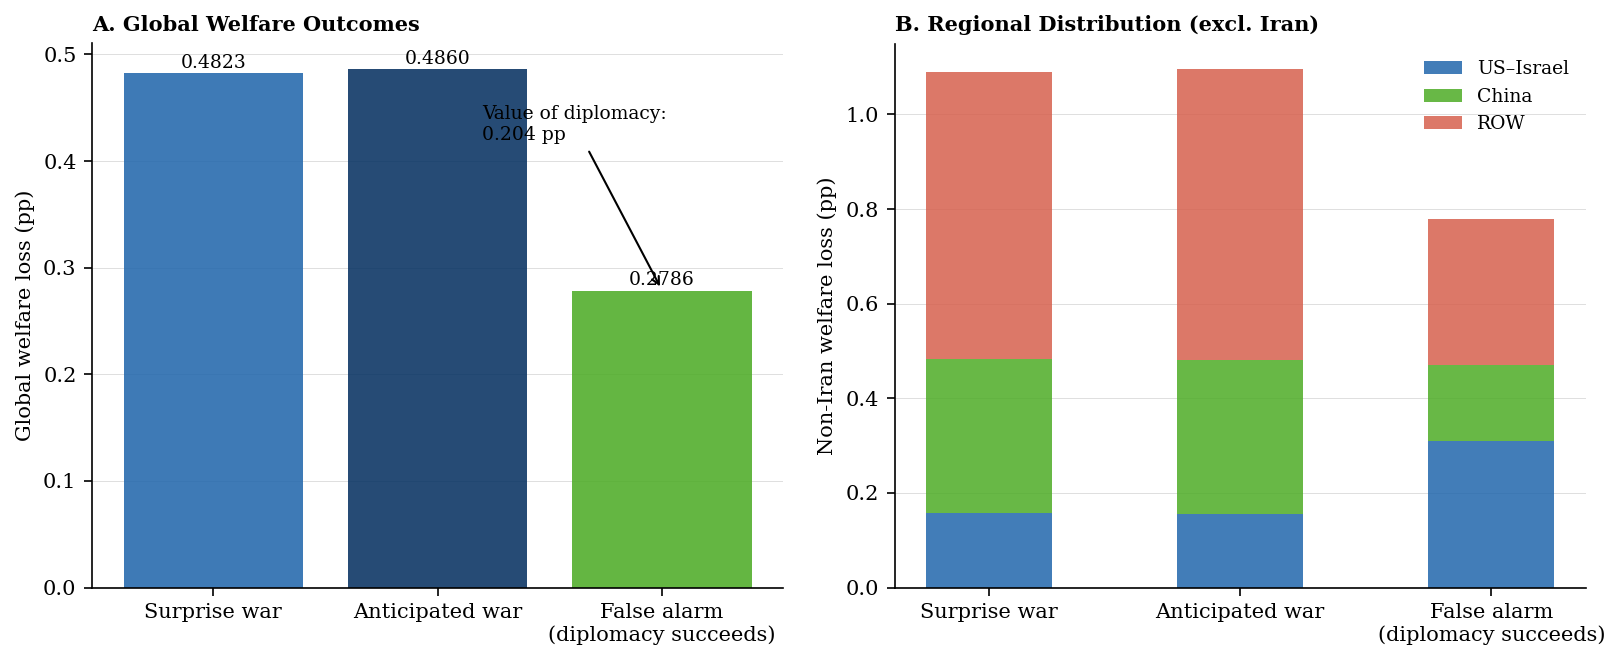
\includegraphics[width=0.85\textwidth]{figures/s4_fig3_news_diplomacy.png}
\caption{Welfare Outcomes and the Value of Diplomacy}
\label{fig:news_diplomacy}
\end{figure}

\begin{table}[H]
\centering
\small
\begin{threeparttable}
\caption{News-Shock Welfare Outcomes}
\label{tab:news}
\begin{tabular}{@{}lccccc@{}}
\toprule
Scenario & Global & Iran & US-Israel & China & ROW \\
\midrule
Surprise war & $+0.4823$pp & $+3.469$pp & $+0.157$pp & $+0.325$pp & $+0.608$pp \\
Anticipated war & $+0.4860$pp & $+3.524$pp & $+0.155$pp & $+0.326$pp & $+0.614$pp \\
False alarm & $+0.2786$pp & $+0.302$pp & $+0.309$pp & $+0.161$pp & $+0.308$pp \\
\bottomrule
\end{tabular}
\begin{tablenotes}[flushleft]
\small
\item Notes: The value of diplomacy, measured as surprise-war loss minus false-alarm loss, is 0.2036pp of global permanent consumption.
\end{tablenotes}
\end{threeparttable}
\end{table}

Anticipation redistributes losses intertemporally but does not substantially alter their total magnitude: the anticipated-war loss (0.486 percentage points) barely exceeds the surprise-war loss (0.482 percentage points), as financial markets partially price in the shock in advance but the realized physical disruption determines the bulk of the welfare cost. The false-alarm scenario, by contrast, yields a welfare loss of only 0.279 percentage points, concentrated in the pre-war financial adjustment costs that unwind when diplomacy succeeds. Diplomacy therefore generates its welfare gains primarily by avoiding the physical oil-supply disruption, not by eliminating pre-war financial turbulence.

\subsection{Inflation-Expectation De-anchoring}
\label{sec:deanchoring}

Expectation de-anchoring is modeled through the backward-looking weight $\lambda$ in equation~(\ref{eq:deanchoring}), crossed with three Taylor-rule inflation-response intensities ($\phi_\pi \in \{1.0, 1.5, 2.5\}$). This two-dimensional comparison tests the central question for monetary policy in a supply-driven energy shock: does more aggressive rate-setting help or harm when expectations are backward-looking?

\begin{figure}[H]
\centering
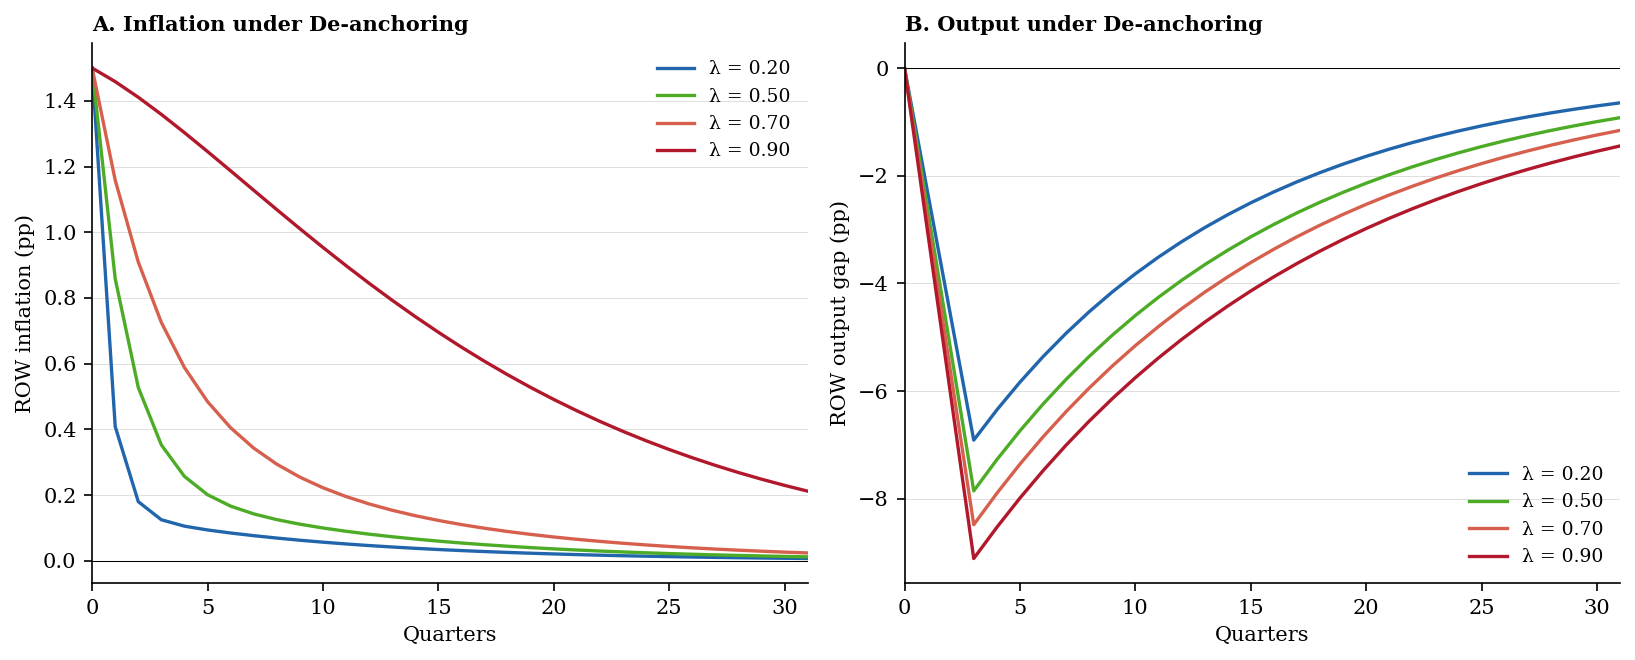
\includegraphics[width=\textwidth]{figures/s5_fig1_deanchoring_paths.png}
\caption{Inflation and Output under Expectation De-anchoring}
\label{fig:deanchoring_paths}
\end{figure}

\begin{figure}[H]
\centering
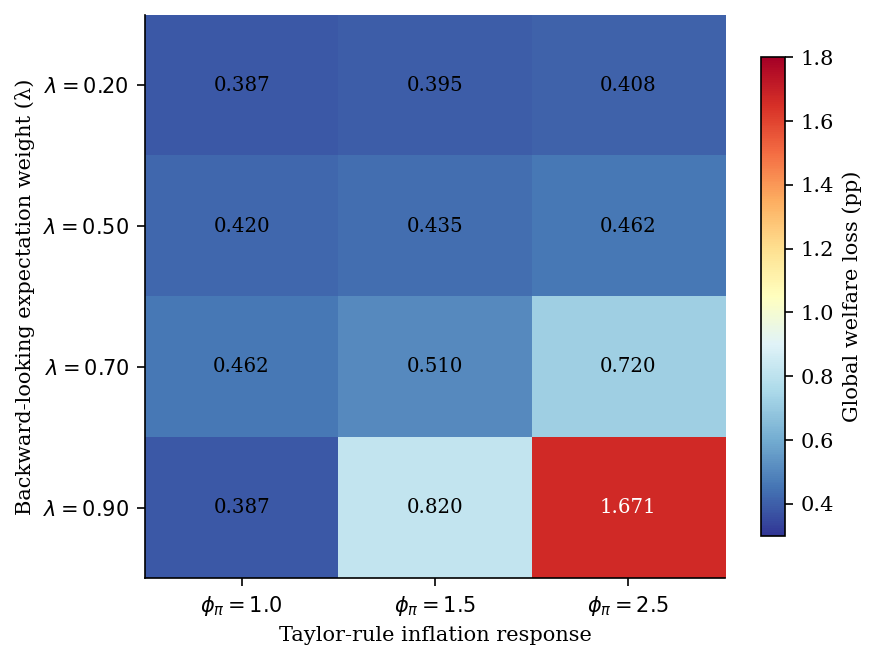
\includegraphics[width=0.8\textwidth]{figures/s5_fig2_deanchoring_heatmap.png}
\caption{Welfare Surface: Backward-Looking Weight and Taylor-Rule Intensity}
\label{fig:deanchoring_heatmap}
\end{figure}

The welfare surface is non-monotone in monetary aggression. Under fully anchored expectations ($\lambda=0.20$), varying $\phi_\pi$ across the three Taylor-rule intensities moves global welfare by less than 0.05 percentage points; monetary activism is nearly irrelevant when credibility is intact. Under severe de-anchoring ($\lambda=0.90$), the hawkish rule ($\phi_\pi=2.5$) produces a 1.6711 percentage-point global welfare loss while the dovish rule ($\phi_\pi=1.0$) produces only 0.3872 percentage points. The maximum de-anchoring cost reaches 1.0996 percentage points in the hawkish column. The explanation is that in an energy supply shock, aggressive rate increases depress output without reducing the cost-push source of inflation; when expectations are backward-looking, this policy configuration amplifies both the output contraction and the inflation spiral rather than attenuating either. Credibility, anchoring $\lambda$ near zero, dominates mechanical Taylor-rule activism as a policy instrument in this environment.

\subsection{Fiscal Sustainability and Debt Dynamics}
\label{sec:debt}

The fiscal exercise studies budget rules under war-driven sovereign spread widening. We compare passive automatic stabilizers, threshold-triggered austerity, and output-gap stimulus against the 130 percent debt-to-GDP sustainability threshold. The exercise asks whether fiscal activism offsets the demand contraction or prevents debt sustainability from binding.

\begin{figure}[H]
\centering
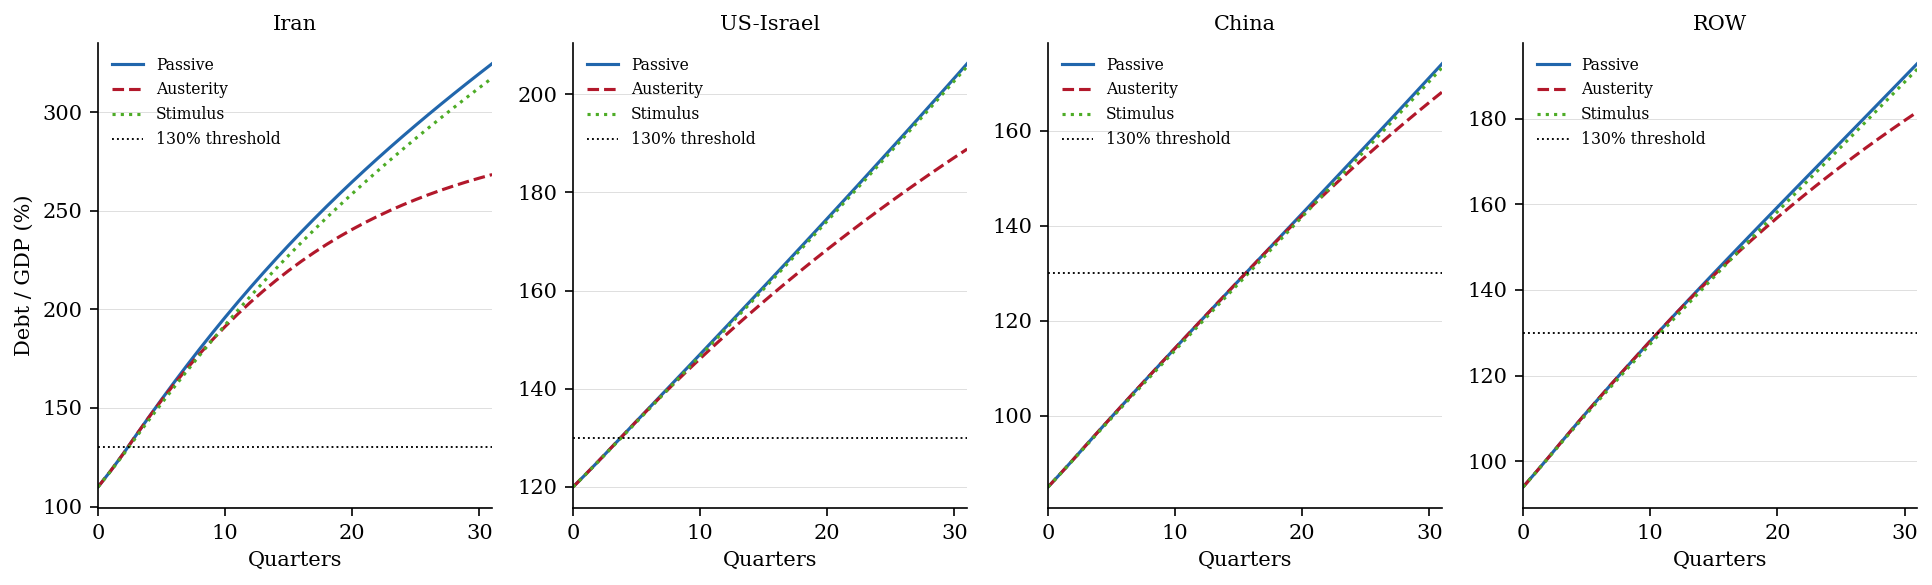
\includegraphics[width=\textwidth]{figures/s6_fig1_debt_paths.png}
\caption{Debt-to-GDP Paths under Fiscal Rules}
\label{fig:debt_paths}
\end{figure}

\begin{figure}[H]
\centering
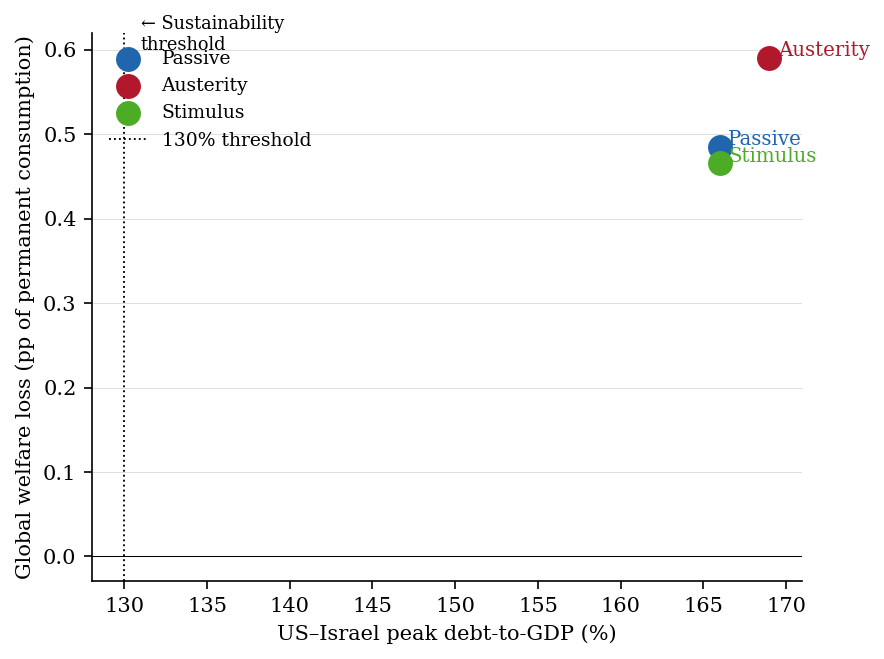
\includegraphics[width=0.9\textwidth]{figures/s6_fig3_debt_fiscal_tradeoff.png}
\caption{Fiscal Welfare--Debt Tradeoff}
\label{fig:debt_tradeoff}
\end{figure}

\begin{table}[H]
\centering
\small
\begin{threeparttable}
\caption{Fiscal Rule Outcomes}
\label{tab:debt}
\begin{tabular}{@{}lccccc@{}}
\toprule
Fiscal rule & Global welfare & Iran debt & US-Israel debt & China debt & ROW debt \\
\midrule
Passive & $+0.4850$pp & $110\%$ & $166\%$ & $87\%$ & $96\%$ \\
Austerity & $+0.5907$pp & $110\%$ & $169\%$ & $87\%$ & $96\%$ \\
Stimulus & $+0.4653$pp & $107\%$ & $166\%$ & $87\%$ & $95\%$ \\
\bottomrule
\end{tabular}
\begin{tablenotes}[flushleft]
\small
\item Notes: Debt entries are peak debt-to-GDP ratios. US-Israel breaches the 130 percent threshold under all three rules.
\end{tablenotes}
\end{threeparttable}
\end{table}

Fiscal stimulus modestly improves welfare relative to the passive baseline (0.465 versus 0.485 percentage points), while austerity worsens it (0.591 percentage points) by compounding the demand contraction through a procyclical fiscal multiplier. Critically, none of the three rules prevents the US--Israel bloc from breaching the 130 percent sustainability threshold: the combination of high initial debt, rising spreads, and the endogenous spread-debt feedback loop in equation~(\ref{eq:debt}) ensures that the bloc crosses the threshold under every fiscal response. This finding implies that debt sustainability in the US--Israel bloc is a function of pre-shock fiscal space, not of the crisis-response rule chosen, and that rebuilding fiscal capacity before geopolitical shocks materialize is the operative margin for reducing fiscal tail risk.

\FloatBarrier

% ============================================================================
% VI. CONCLUSION
% ============================================================================

\section{Conclusion}
\label{sec:conclusion}

This paper studies a rare geopolitical disaster, a Strait of Hormuz blockade, that converts a localized military escalation into a global macroeconomic shock through the world's most concentrated energy transit node. The analysis is deliberately structural: rather than estimating an average war effect, the model isolates the oil-supply shock, financial contagion, trade disruption, stabilization policy, expectation dynamics, and fiscal sustainability channels that jointly determine the path of output, inflation, and welfare across four world regions. The central finding is that a Hormuz closure is not well approximated by either a standard oil-supply shock or a standard war shock. In the baseline path, the blockade raises global oil prices by 64.2 percent, pushes Iran's output gap to $-34.1$ percentage points, and generates a global consumption-equivalent welfare loss of 0.485 percentage points of permanent consumption. The global aggregate, however, conceals the economics that matter most for policy: losses are concentrated at the war site and among oil-importing third countries, while oil exporters within the aggregate ROW block are nearly insulated by their terms-of-trade windfall.

The transmission structure also reshapes the policy ranking. China's triple stabilization reduces the oil-price peak by about five percentage points and lowers the global welfare loss by 0.045 percentage points, but the OPEC+ extension demonstrates that spare physical production capacity is the larger marginal stabilizer in the oil-price channel. This does not render China's instruments peripheral: the two sets of tools stabilize qualitatively different margins. OPEC+ acts directly on the missing-barrel supply gap; China's SPR, renewable substitution, and manufacturing expansion operate through reserve smoothing, import-cost pass-through reduction, and supply-chain substitution. The broader lesson is that a chokepoint disaster activates multiple binding constraints simultaneously, and each policy instrument is effective only at the margin where its constraint is operative. This has direct implications for energy-security investment priorities: marginal returns to additional OPEC+ spare capacity exceed those of additional strategic petroleum reserves for shocks of this type, while China's manufacturing capacity generates global welfare externalities that exceed those of reserve expansion.

The six counterfactual exercises reinforce and sharpen this message. Disaggregating ROW reveals that the aggregate third-country block mixes nearly insulated oil exporters with much more vulnerable oil importers, so global welfare averages systematically understate the distributional severity of the shock. Escalation to Gulf infrastructure damage moves the model into a strongly convex nonlinear tail. Severe escalation raises the oil-price peak to 126.6 percent and global welfare losses to 0.731 percentage points, 51 percent above the baseline. The news-shock exercise demonstrates that geopolitical threats impose real welfare costs before physical disruption occurs through financial-market pre-adjustment, while successful diplomacy avoids 0.204 percentage points of global permanent consumption loss by removing the physical disruption entirely. The de-anchoring and debt exercises identify the two binding second-round policy risks: when inflation expectations become sufficiently backward-looking, aggressive Taylor-rule tightening worsens welfare by amplifying output contractions without reducing the cost-push source of inflation; and when initial government debt is elevated, the endogenous spread--debt feedback loop converts a short-run energy shock into a medium-run fiscal sustainability crisis that no crisis-era fiscal rule can prevent.

These results reframe the standard demand-management interpretation of crisis policy. The problem posed by a Hormuz blockade is not a uniform shortfall of aggregate demand. Different parts of the global economy face qualitatively distinct constraints: some are supply-constrained by missing barrels, some are financially constrained by elevated risk premia and capital flight, and some are fiscally constrained by rising debt-service costs. Interest-rate policy can influence the path of inflation and output gaps, but it cannot produce oil, reopen a chokepoint, or eliminate sovereign-spread contagion. The policy priorities implied by the model are accordingly concrete: anchor inflation expectations before a crisis to avoid the welfare trap documented in the de-anchoring exercise; maintain spare oil-supply capacity across multiple geographic nodes to ensure OPEC+ has the market power to respond effectively; direct financial stabilization support toward oil-importing economies, which bear the distributional burden concealed by aggregate ROW figures; and restore fiscal space during peacetime rather than attempting to rebuild it after spreads have already widened and the debt-sustainability feedback loop has engaged.

The central finding---that sovereign credit risk network contagion amplifies traditional trade-channel losses by a quantitatively large margin---is established by comparing the model's financial-channel-on versus financial-channel-off configurations, rather than by the level of any single welfare number. This comparative design insulates the core result from the most consequential limitation of the framework: the financial-channel equations are reduced-form approximations to BGG-style financial accelerator dynamics, calibrated to match historical geopolitical-stress episodes but not estimated from those episodes via a structural identification scheme. The model also does not impose a full system of bilateral current-account and goods-market clearing conditions, with trade disruptions entering as calibrated wedges rather than endogenously determined import-demand schedules. China's stabilization deployment paths are derived as solutions to the constrained policy optimization problem~(\ref{eq:china_opt})--(\ref{eq:mfg_cap}), ensuring internal consistency with the optimization framework, though the cost parameters $c_s$, $c_r$, and $c_m$ are calibrated rather than estimated. These limitations circumscribe the strongest quantitative claims: the paper speaks most confidently to the relative magnitudes of oil, financial, expectation, and fiscal channels and to the ordering of stabilization instruments by effectiveness, both of which are robust to reasonable re-calibration of parameters the paper does not estimate.

Three extensions are the most valuable next steps. First, the financial linkage matrix should be formally estimated rather than calibrated, using a structural VAR identified by geopolitical risk shocks on higher-frequency sovereign CDS, equity index, and capital-flow data from historical geopolitical stress episodes; the GPR index of \citet{caldara2022measuring} provides a natural external instrument, and Bayesian estimation would deliver posterior distributions for each $L_{ij}$ that could be used to construct credible intervals around the paper's welfare calculations. Second, the ROW exporter--importer disaggregation should be embedded in the baseline with endogenous current-account clearing and exchange-rate adjustment, allowing the terms-of-trade redistribution between the two subgroups to feed back into global demand in a way the current calibrated-wedge specification cannot. Third, OPEC+ spare capacity release and diplomatic conflict prevention should be incorporated as additional strategic choices in the policy optimization framework developed in Section~\ref{sec:china}, extending the constrained planner problem~(\ref{eq:china_opt})--(\ref{eq:mfg_cap}) into a multi-player game with endogenous coordination costs and political-economy constraints, transforming the paper's counterfactual comparisons into a formal mechanism-design problem.

% ============================================================================
% REFERENCES
% ============================================================================

\newpage
\bibliographystyle{aer}

\begin{thebibliography}{99}

\bibitem[Abadie and Gardeazabal(2003)]{abadie2003economic}
Abadie, Alberto, and Javier Gardeazabal. 2003. ``The Economic Costs of Conflict: A Case Study of the Basque Country.'' \textit{American Economic Review}, 93(1): 113--132.

\bibitem[Autor, Dorn, and Hanson(2013)]{autor2013china}
Autor, David H., David Dorn, and Gordon H. Hanson. 2013. ``The China Syndrome: Local Labor Market Effects of Import Competition in the United States.'' \textit{American Economic Review}, 103(6): 2121--2168.

\bibitem[Barro(2006)]{barro2006rare}
Barro, Robert J. 2006. ``Rare Disasters and Asset Markets in the Twentieth Century.'' \textit{Quarterly Journal of Economics}, 121(3): 823--866.

\bibitem[Bernanke, Gertler, and Gilchrist(1999)]{bernanke1999financial}
Bernanke, Ben S., Mark Gertler, and Simon Gilchrist. 1999. ``The Financial Accelerator in a Quantitative Business Cycle Framework.'' In \textit{Handbook of Macroeconomics}, edited by John B. Taylor and Michael Woodford, Vol.~1, 1341--1393. Amsterdam: Elsevier.

\bibitem[Bernanke(2005)]{bernanke2005global}
Bernanke, Ben S. 2005. ``The Global Saving Glut and the U.S.\ Current Account Deficit.'' Sandridge Lecture, Virginia Association of Economists.

\bibitem[Blanchard and Gal\'{i}(2007)]{blanchard2007macroeconomic}
Blanchard, Olivier J., and Jordi Gal\'{i}. 2007. ``The Macroeconomic Effects of Oil Price Shocks: Why Are the 2000s So Different from the 1970s?'' NBER Working Paper 13368.

\bibitem[Bodenstein, Erceg, and Guerrieri(2011)]{bodenstein2011oil}
Bodenstein, Martin, Christopher J. Erceg, and Luca Guerrieri. 2011. ``Oil Shocks and External Adjustment.'' \textit{Journal of International Economics}, 83(2): 168--184.

\bibitem[Borensztein and Panizza(2013)]{borensztein2013debt}
Borensztein, Eduardo, and Ugo Panizza. 2013. ``The Costs of Sovereign Default.'' \textit{IMF Staff Papers}, 56(4): 683--741.

\bibitem[Caldara and Iacoviello(2022)]{caldara2022measuring}
Caldara, Dario, and Matteo Iacoviello. 2022. ``Measuring Geopolitical Risk.'' \textit{American Economic Review}, 112(4): 1194--1225.

\bibitem[{Energy Information Administration}(2023)]{eia2023hormuz}
Energy Information Administration. 2023. ``The Strait of Hormuz Is the World's Most Important Oil Transit Chokepoint.'' EIA Today in Energy, June 20.

\bibitem[Federle et~al.(2026)]{federle2026price}
Federle, Jonathan, Andr\'{e} Meier, Gernot J. M\"{u}ller, Willi Mutschler, and Moritz Schularick. 2026. ``The Price of War.'' \textit{American Economic Review}, 116(3): 791--827.

\bibitem[Gal\'{i}(2015)]{gali2015monetary}
Gal\'{i}, Jordi. 2015. \textit{Monetary Policy, Inflation, and the Business Cycle: An Introduction to the New Keynesian Framework}. 2nd ed. Princeton: Princeton University Press.

\bibitem[Hamilton(1983)]{hamilton1983oil}
Hamilton, James D. 1983. ``Oil and the Macroeconomy since World War II.'' \textit{Journal of Political Economy}, 91(2): 228--248.

\bibitem[Hamilton(2009)]{hamilton2009understanding}
Hamilton, James D. 2009. ``Understanding Crude Oil Prices.'' \textit{Energy Journal}, 30(2): 179--206.

\bibitem[Helveston et~al.(2022)]{helveston2019china}
Helveston, John Paul, Gang He, and Michael R. Davidson. 2022. ``Quantifying the Cost Savings of Global Solar Photovoltaic Supply Chains.'' \textit{Nature}, 612: 83--87.

\bibitem[Hilscher and Nosbusch(2010)]{hilscher2010determinants}
Hilscher, Jens, and Yves Nosbusch. 2010. ``Determinants of Sovereign Risk: Macroeconomic Fundamentals and the Pricing of Sovereign Debt.'' \textit{Review of Finance}, 14(2): 235--262.

\bibitem[Jord\`{a}(2005)]{jorda2005estimation}
Jord\`{a}, \`{O}scar. 2005. ``Estimation and Inference of Impulse Responses by Local Projections.'' \textit{American Economic Review}, 95(1): 161--182.

\bibitem[Kilian(2009)]{kilian2009not}
Kilian, Lutz. 2009. ``Not All Oil Price Shocks Are Alike: Disentangling Demand and Supply Shocks in the Crude Oil Market.'' \textit{American Economic Review}, 99(3): 1053--1069.

\bibitem[Longstaff et~al.(2011)]{longstaff2011financial}
Longstaff, Francis A., Jun Pan, Lasse H. Pedersen, and Kenneth J. Singleton. 2011. ``How Sovereign Is Sovereign Credit Risk?'' \textit{American Economic Journal: Macroeconomics}, 3(2): 75--103.

\bibitem[Lucas(1987)]{lucas1987models}
Lucas, Robert E., Jr. 1987. \textit{Models of Business Cycles}. Oxford: Basil Blackwell.

\bibitem[Ramey(2011)]{ramey2011identifying}
Ramey, Valerie A. 2011. ``Identifying Government Spending Shocks: It's All in the Timing.'' \textit{Quarterly Journal of Economics}, 126(1): 1--50.

\bibitem[Rey(2015)]{rey2015dilemma}
Rey, H\'{e}l\`{e}ne. 2015. ``Dilemma Not Trilemma: The Global Financial Cycle and Monetary Policy Independence.'' NBER Working Paper 21162.

\bibitem[Zhang et~al.(2020)]{zhang2020china}
Zhang, Dayong, Qiang Ji, and Apostolos Kiohos. 2020. ``China's Oil Strategic Petroleum Reserve: A DSGE Analysis.'' \textit{Energy Economics}, 88: 104748.

\end{thebibliography}

% ============================================================================
% APPENDIX (FOR ONLINE PUBLICATION)
% ============================================================================

\newpage
\appendix
\section*{Appendix: Model Equations Summary}
\addcontentsline{toc}{section}{Appendix}

For reference, we collect the complete system of equations for each region $i$:

\begin{align}
\pi_{i,t} &= \beta \pi^e_{i,t} + \kappa_i \, \hat{y}_{i,t-1} + 0.25\,\alpha_{e,i}\Delta p^{\text{oil}}_t + 0.40\,\delta^{\text{destroy}}_{i,t} - 0.10\,\chi^{\text{mfg}}_t\omega_i \tag{A.1} \\[6pt]
\hat{y}_{i,t} &= \rho \, \hat{y}_{i,t-1} - \frac{1}{\sigma_i}(i_{i,t} - \pi^e_{i,t}) + 0.8 \, g^{\text{mil}}_{i,t} - \tau^{\text{trade}}_{i,t} - 0.15 \, \alpha_{e,i} \Delta p^{\text{oil}}_t + \Phi^{\text{fin}}_{i,t} \tag{A.2} \\[6pt]
i_{i,t} &= \rho_{i,i} \, i_{i,t-1} + (1-\rho_{i,i})(\phi_{\pi,i} \pi_{i,t} + \phi_{y,i} \hat{y}_{i,t-1}) \tag{A.3} \\[6pt]
s_{i,t} &= s^{\text{shock}}_{i,t} + 0.3 \max(-\hat{y}_{i,t-1}, 0) + 0.2 \, s_{i,t-1} \tag{A.4} \\[6pt]
k_{i,t} &= k^{\text{shock}}_{i,t} - 2 s_{i,t} + 0.5(i_{i,t} - 0.02) + 0.3 \, k_{i,t-1} \tag{A.5} \\[6pt]
q_{i,t} &= 0.6 \, q_{i,t-1} + 10 g^e_{i,t} - 8(i_{i,t} + s_{i,t}) - 3 \max(-\hat{y}_{i,t},0) + q^{\text{shock}}_{i,t} \tag{A.6} \\[6pt]
e_{i,t} &= 0.4 \, e_{i,t-1} + 0.5 \, s_{i,t} - 0.3 \, k_{i,t} + \iota^{\text{fx}}_{i,t} \tag{A.7} \\[6pt]
\Phi^{\text{fin}}_{i,t} &= -0.15 \, s_{i,t} - 0.10 \max(-k_{i,t}, 0) \tag{A.8}
\end{align}

The global oil market clears according to:
\begin{align}
\Delta S_t &= \lambda^{\text{block}}_t (s^H - s^{\text{Iran}}) + s^{\text{Iran}}\lambda^{\text{prod}}\frac{\lambda^{\text{block}}_t}{0.70} - 0.30 \lambda^{\text{block}}_t (s^H - s^{\text{Iran}}) \tag{A.9} \\[6pt]
\Delta p^{\text{oil},*}_t &= \max\left\{\frac{\Delta S_t-\text{SPR}^{\text{China}}_t-\text{SPR}^{\text{US}}_t-\text{OPEC}_t+\Delta D_t}{|\varepsilon_d|+\varepsilon_s},0\right\} \tag{A.10}\\[6pt]
\Delta p^{\text{oil}}_t &=0.15\,\Delta p^{\text{oil}}_{t-1}+0.85\,\Delta p^{\text{oil},*}_t \tag{A.11}
\end{align}

Financial contagion operates through:
\begin{equation}
\tilde{s}^{\text{shock}}_{j,t} = s^{\text{shock}}_{j,t} + 0.1 \Big(\textstyle\sum_{i \neq j} L_{ij} s_{i,t-1}\Big)(1 + 2\max(-k_{\text{Iran},t}, 0)) \tag{A.12}
\end{equation}

\end{document}
